% ADF
% version 2018
%-------------------------------------------------------

% Ver el siguiente link para ecuaciones de maxwell

% http://www.librosmaravillosos.com/17ecuacionesquecambiaronelmundo/index.html#capitulo11

% y este otro

% http://irregularwebcomic.net/1420.html

% Una regla mnemotecnica para las ecuaciones de maxwell

% https://borrowbits.com/2012/05/aprender-las-leyes-de-maxwell-con-una-sola-mano/

%http://www.wolfram-stanek.de/maxwell/maxwell_hand.htm


\section{Introducci\'on}

Como su nombre lo indica, las radioayudas basan su funcionamiento en las ondas de radio,
por ello es conveniente comenzar explicando los conceptos b\'asicos asociados a las ondas en general y a las ondas electromagn\'eticas en particular (de las cuales las ondas de radio son apenas un subconjunto).

Posteriormente se describe uno de los primeros sistemas de radioayudas, que a\'un hoy se encuentra en uso, el LORAN.

Finalmente se describe un sistema posterior de radioayuda, el ADF.

\section{ Ondas Electromagn\'eticas }

\subsection{Caracter\'isticas generales}

En este sentido, es menester empezar definiendo lo que es una onda electromagn\'etica: es un tipo de radiaci\'on en forma de onda que se caracteriza por poseer dos campos: un campo el\'ectrico y otro campo magn\'etico, oscilando perpendicularente entre s\'i. La Figura \ref{fig:onda-electromagnetica} representa una onda electromagn\'etica: 

\begin{figure}[!h]
  \centering
  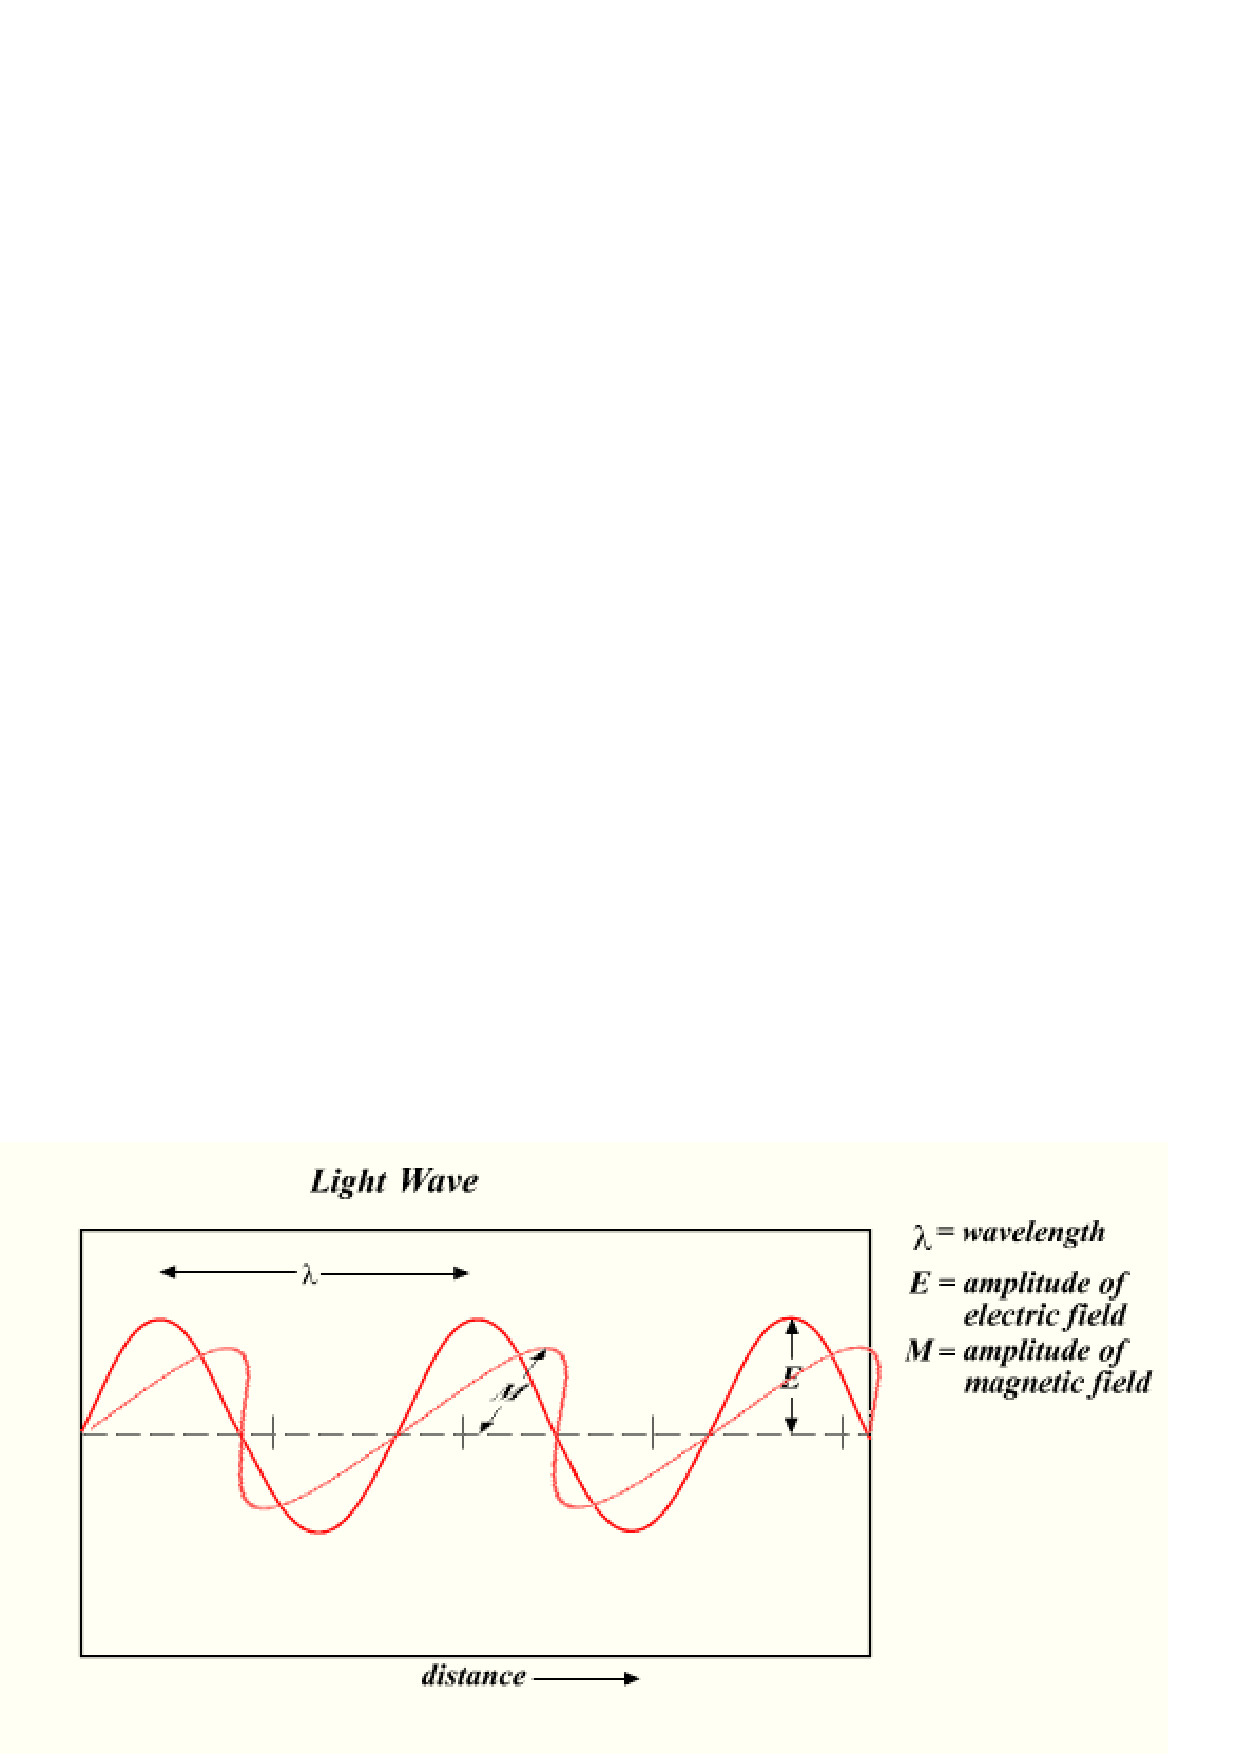
\includegraphics[width=0.7\textwidth]{Imagenes/06.01.adf/onda-electromagnetica.png}  
  \caption{Onda electromagn\'etica \cite{wikipedia_esp}}
  \label{fig:onda-electromagnetica}
\end{figure}

Para entender mejor su comportamiento, se recuerdan los siguientes conceptos:

\begin{description}
\item [Ciclo] Es cada patr\'on repetitivo de una onda.

\item  [Per\'iodo] Tiempo que tarda la onda en completar un ciclo.

\item  [Frecuencia] N\'umero de ciclos que completa la onda en un intervalo de
  tiempo. Si dicho intervalo es de un segundo, la unidad de frecuencia
  es el Hertz (Hz). Otras unidades de frecuencias muy utilizadas (en
  otros \'ambitos) son las ``\textit{revoluciones por minuto}'' (RPM) y los
  ``\textit{radianes por segundo}'' (rad/s).

El per\'iodo y la frecuencia est\'an relacionados como $ f = 1/T $

\item [Amplitud] Es la medida de la magnitud de la m\'axima perturbaci\'on del medio producida por la onda.

\item [Longitud] La longitud de una onda viene determinada por la distancia entre los puntos inicial y final de un ciclo (por ejemplo, entre un valle de la onda y el siguiente). Habitualmente se denota con la letra griega $\lambda$ (lambda).



Un factor importante a tener en cuenta es que el tama\~no y dise\~no de las antenas est\'a fuertemente influenciado por la longitud de onda. Por ejemplo, una antena dipolo sencilla debe tener una longitud $\lambda/2$ para que sintonice de manera \'optima las ondas de longitud $\lambda$.

Los conceptos anteriores est\'an representados en la Figura \ref{fig:propiedades-onda}.

\begin{figure}[!h]
  \centering
 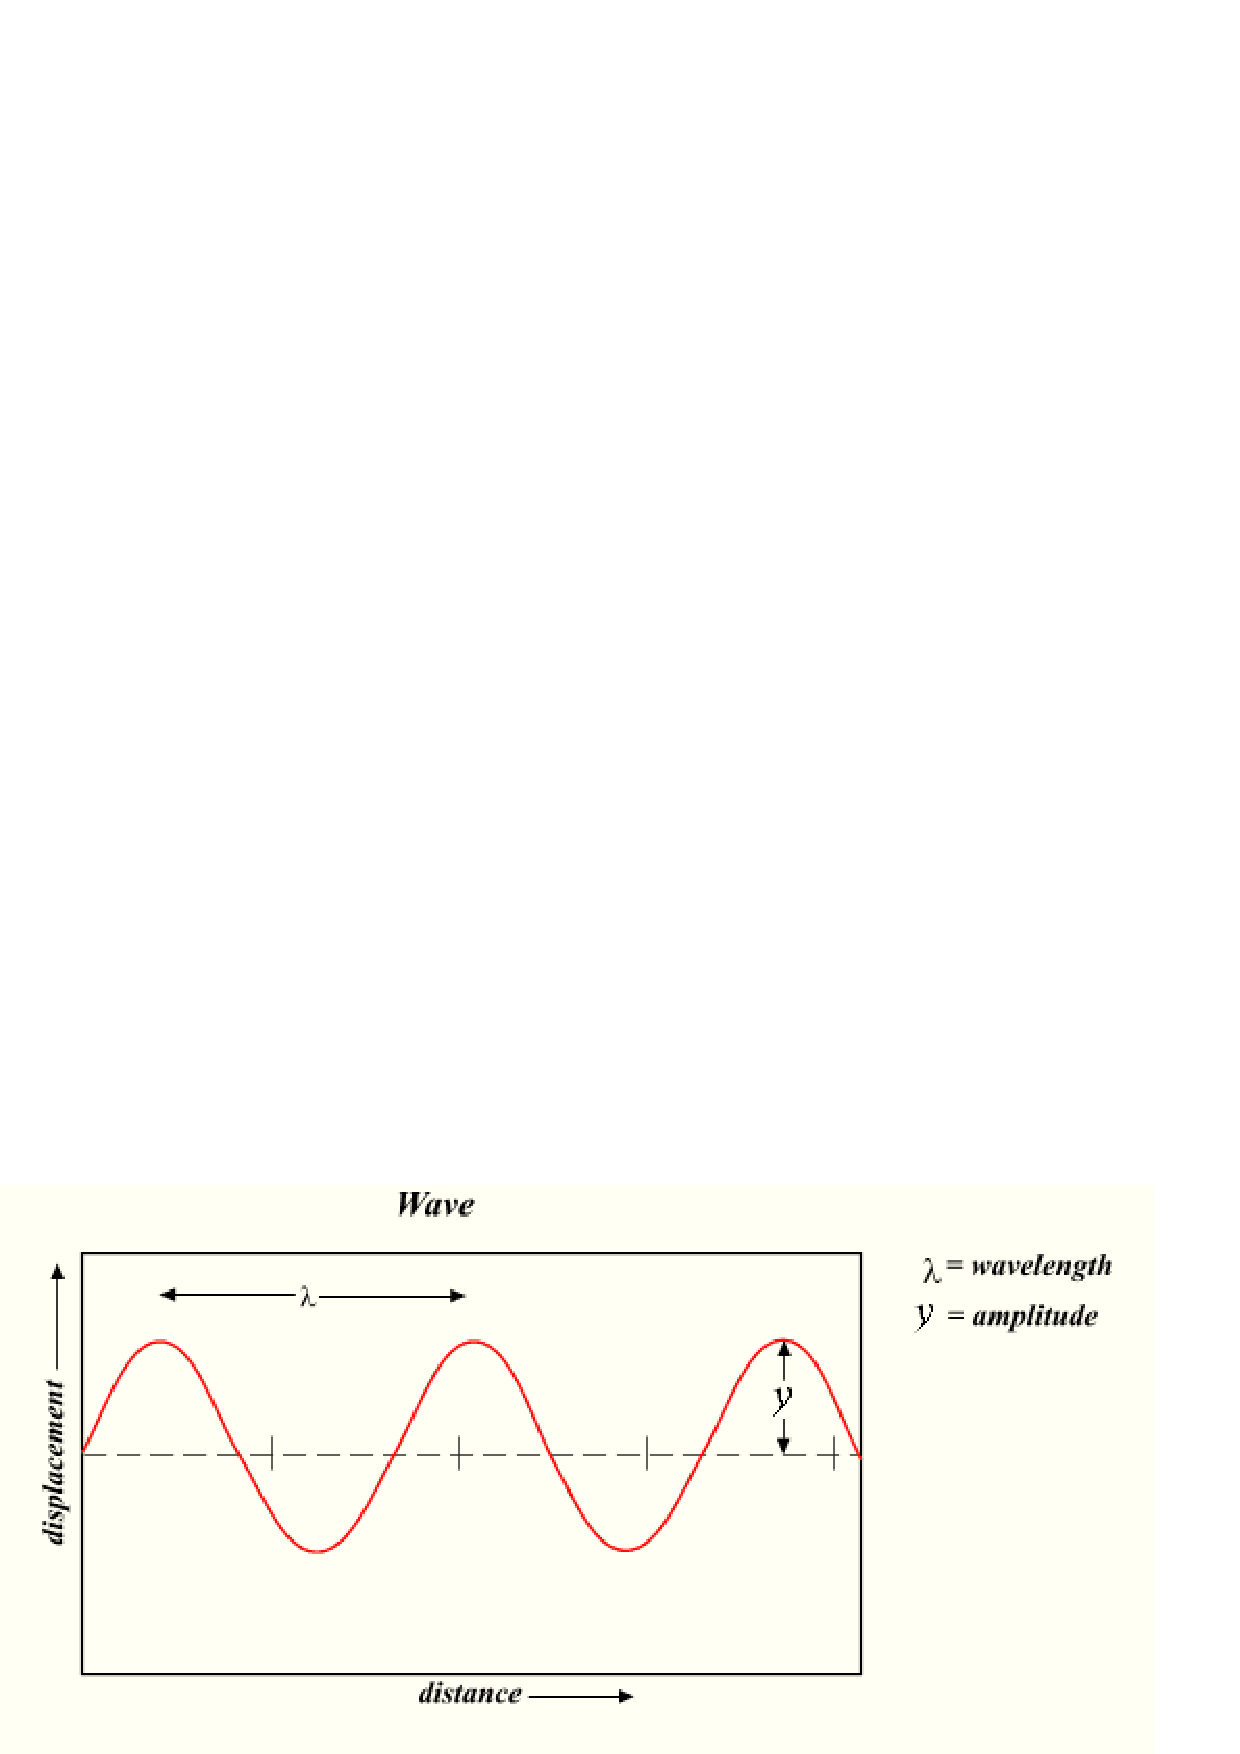
\includegraphics[width=0.7\textwidth]{./Imagenes/06.01.adf/propiedades-onda.png}  
  \caption{Propiedades de una onda \cite{wikipedia_esp}}
  \label{fig:propiedades-onda}
\end{figure}


\item [Velocidad] Las ondas se desplazan a una velocidad que depende de la naturaleza de la onda y del medio por el cual se mueven. En el caso de la luz, por ejemplo, la velocidad en el vac\'io se denota $c$ y vale 299.792.458 m/s (aproximadamente $3 \cdot 10^8 \, m/s$).

Los conceptos de velocidad, longitud y frecuencia est\'an interrelacionados. Para el caso de las ondas electromagn\'eticas (de las cuales la luz es un ejemplo), la relaci\'on se expresa como $ \lambda = c / f $


\item [Fase] La fase de una onda relaciona la posici\'on de una caracter\'istica espec\'ifica del ciclo (como por ejemplo un pico), con la posici\'on de esa misma caracter\'istica en otra onda. Puede medirse en unidades de tiempo, distancia, fracci\'on de la longitud de onda o (m\'as com\'unmente) como un \'angulo.

Tomese en cuenta que la definici\'on de fase lleva impl\'icita la comparaci\'on de dos ondas de la misma frecuencia, pues en caso contrario no tiene mucho sentido dicha comparaci\'on.

La Figura \ref{fig:desfase-ondas} muestra varias ondas con diferentes fases. 

\begin{figure}[!h]
  \centering
  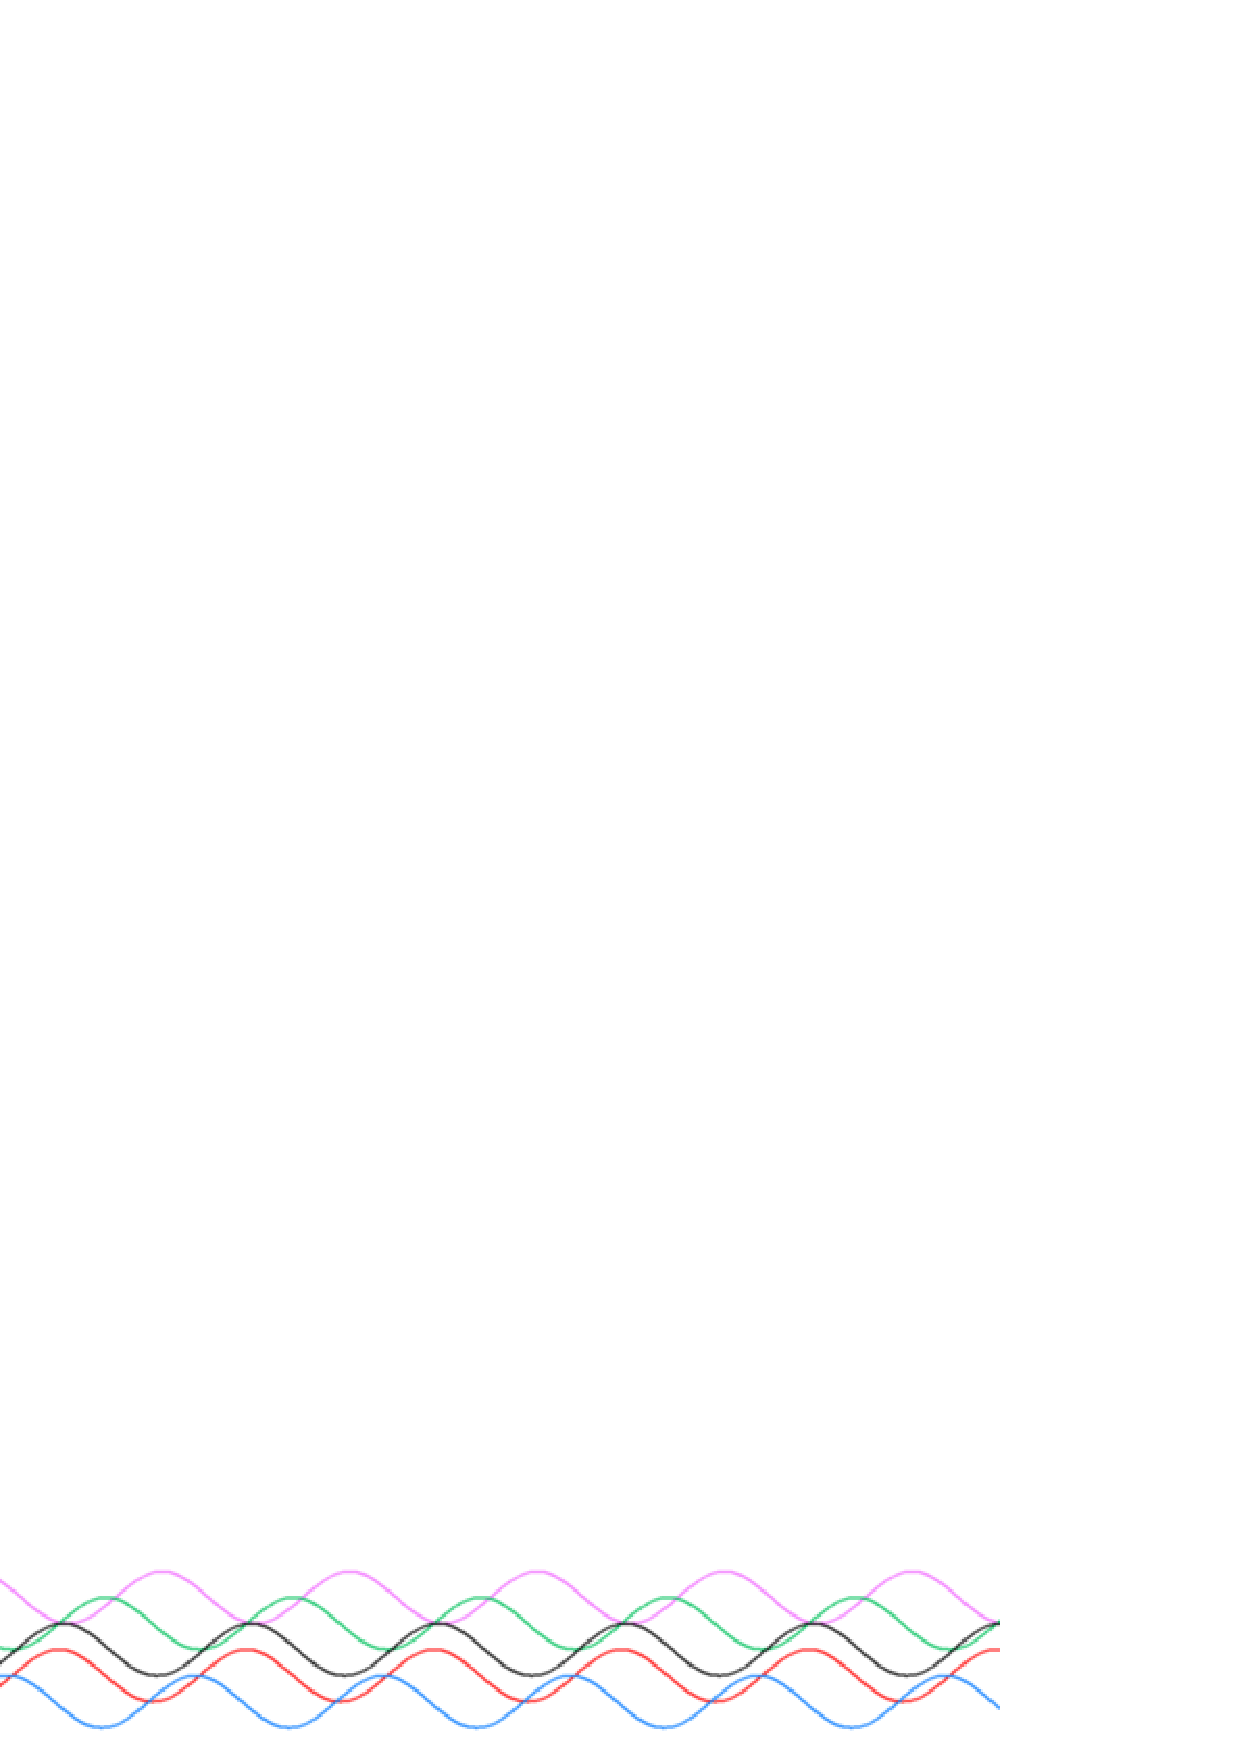
\includegraphics[width=0.7\textwidth]{./Imagenes/06.01.adf/desfase-ondas.png}
  \caption{Ondas con diferentes fases \cite{wikipedia_esp}}
  \label{fig:desfase-ondas}
\end{figure}



\item [Polarizaci\'on] Representa la orientaci\'on con la que la onda oscila, y en el caso particular de las ondas electromagn\'eticas, la orientaci\'on en la oscilaci\'on del campo el\'ectrico. A menudo esta orientaci\'on es una l\'inea y por ello se habla t\'ipicamente de ondas con polarizaci\'on vertical u horizontal, es decir, cuando el campo el\'ectrico oscila en un plano con esas direcciones. 


  \begin{figure}[!h]
    \centering
  \includegraphics[width=0.7\textwidth]{./Imagenes/06.01.adf/polarizacion-ondas.png}    
    \caption{Polarizaci\'on de las ondas electromagn\'eticas \cite{wikipedia_esp}}
    \label{fig:polarizacion-ondas}
  \end{figure}

Adicionalmente, es posible que el campo el\'ectrico cambie su orientaci\'on conforme la onda avanza. Se habla entonces de ondas con polarizaci\'on circular 

\begin{figure}[!h]
  \centering
  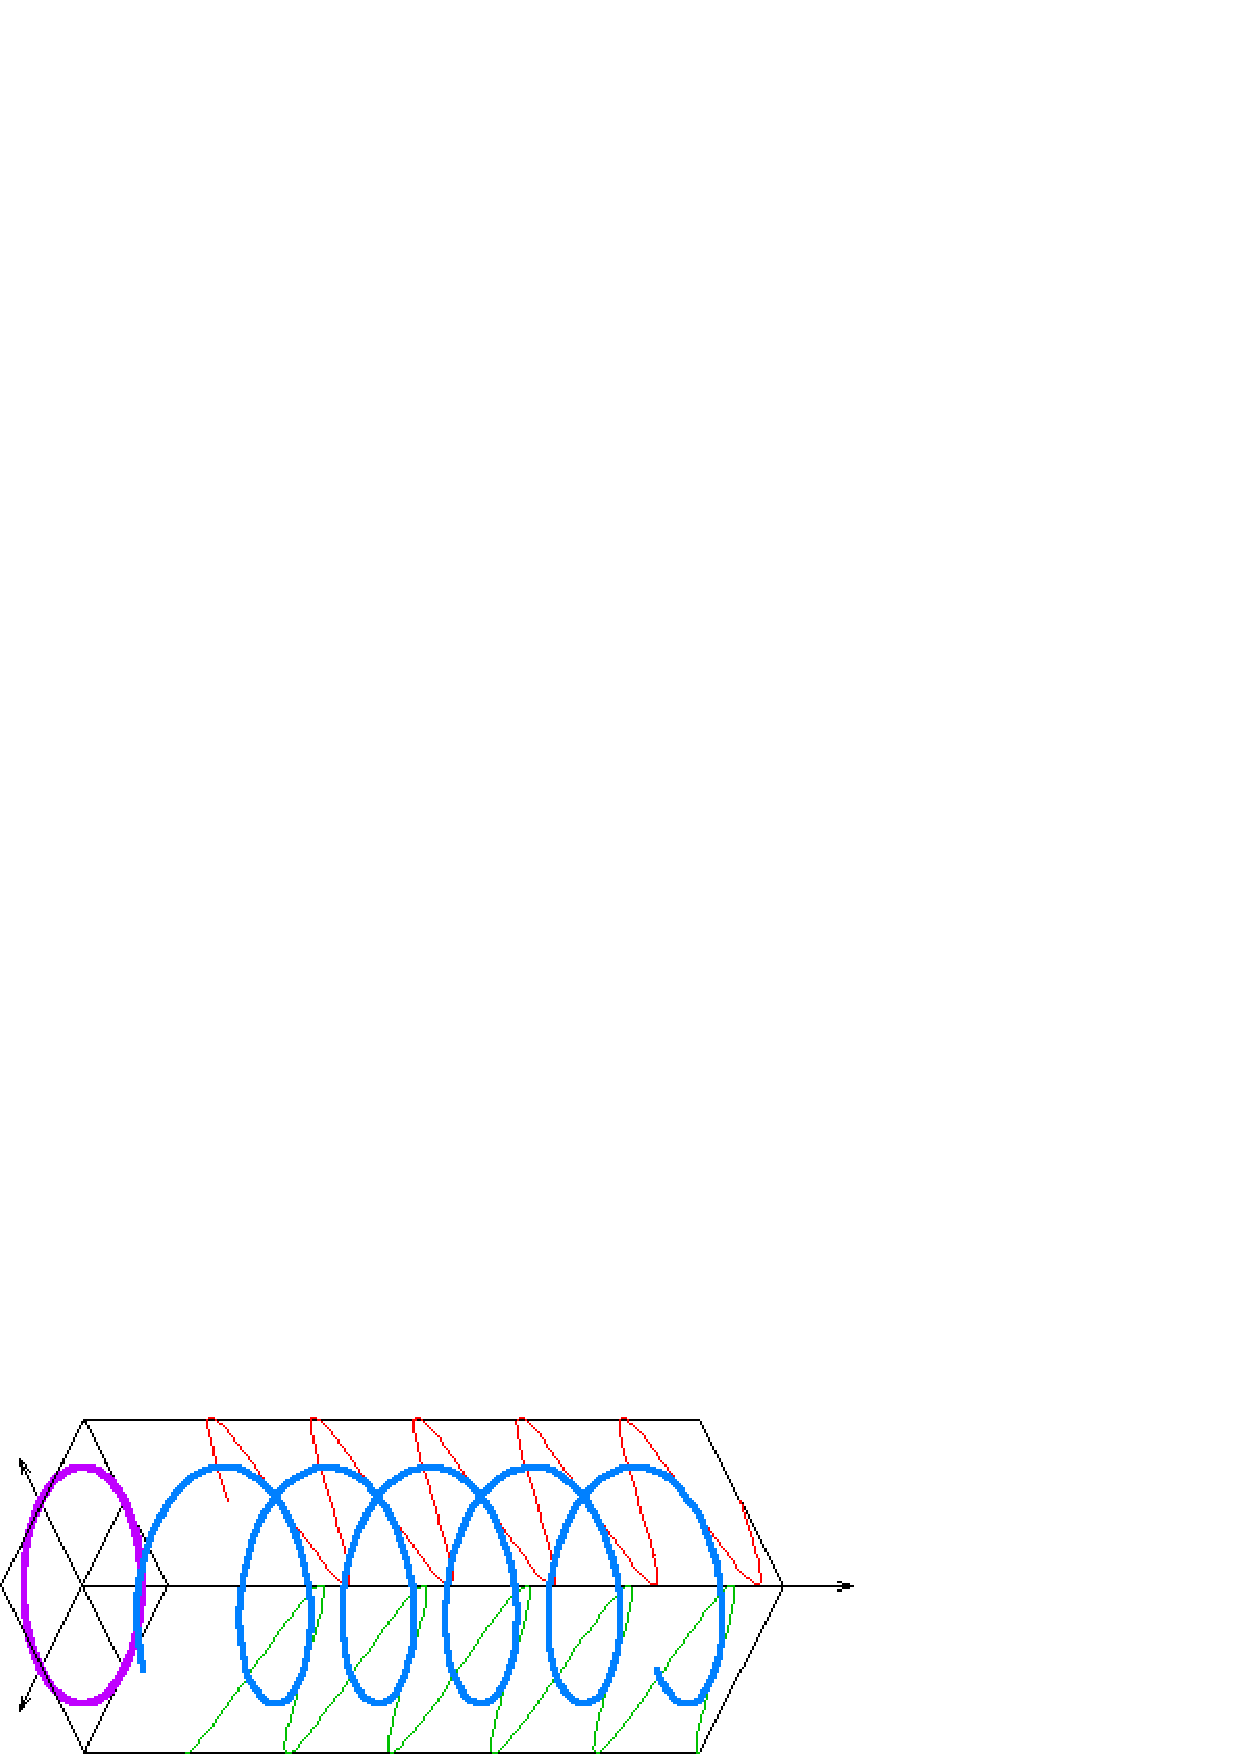
\includegraphics[width=0.7\textwidth]{./Imagenes/06.01.adf/polarizacion-circular.png}  
  \caption{Onda con polarizaci\'on circular \cite{wikipedia_esp}}
  \label{fig:polarizacion-circular}
\end{figure}


\item [Diagramas de radiaci\'on] Las ondas electromagn\'eticas utilizadas por las radioayudas t\'ipicamente se emiten o reciben utilizando diferentes tipos de antenas. Dependiendo del tipo de antena utilizada, la energ\'ia electromagn\'etica puede o no emitirse (o recibirse) con igual intensidad en todas las direcciones.
Se denomina entonces diagrama de radiaci\'on (o emisi\'on) a un diagrama polar que represente la intensidad relativa de la se\~nal electromagn\'etica en funci\'on del azimut alrededor de la antena.
En la Figura \ref{fig:diagramas-radiacion} se presentan dos diagramas de radiaci\'on. El de la izquierda es en forma de ``ocho'' y es muy usado en aviaci\'on, mientras que el de la derecha representa una antena is\'otropa (o no-direccional: aquella cuya emisi\'on o recepci\'on no depende de la direcci\'on). 


\begin{figure}[!h]
  \centering
 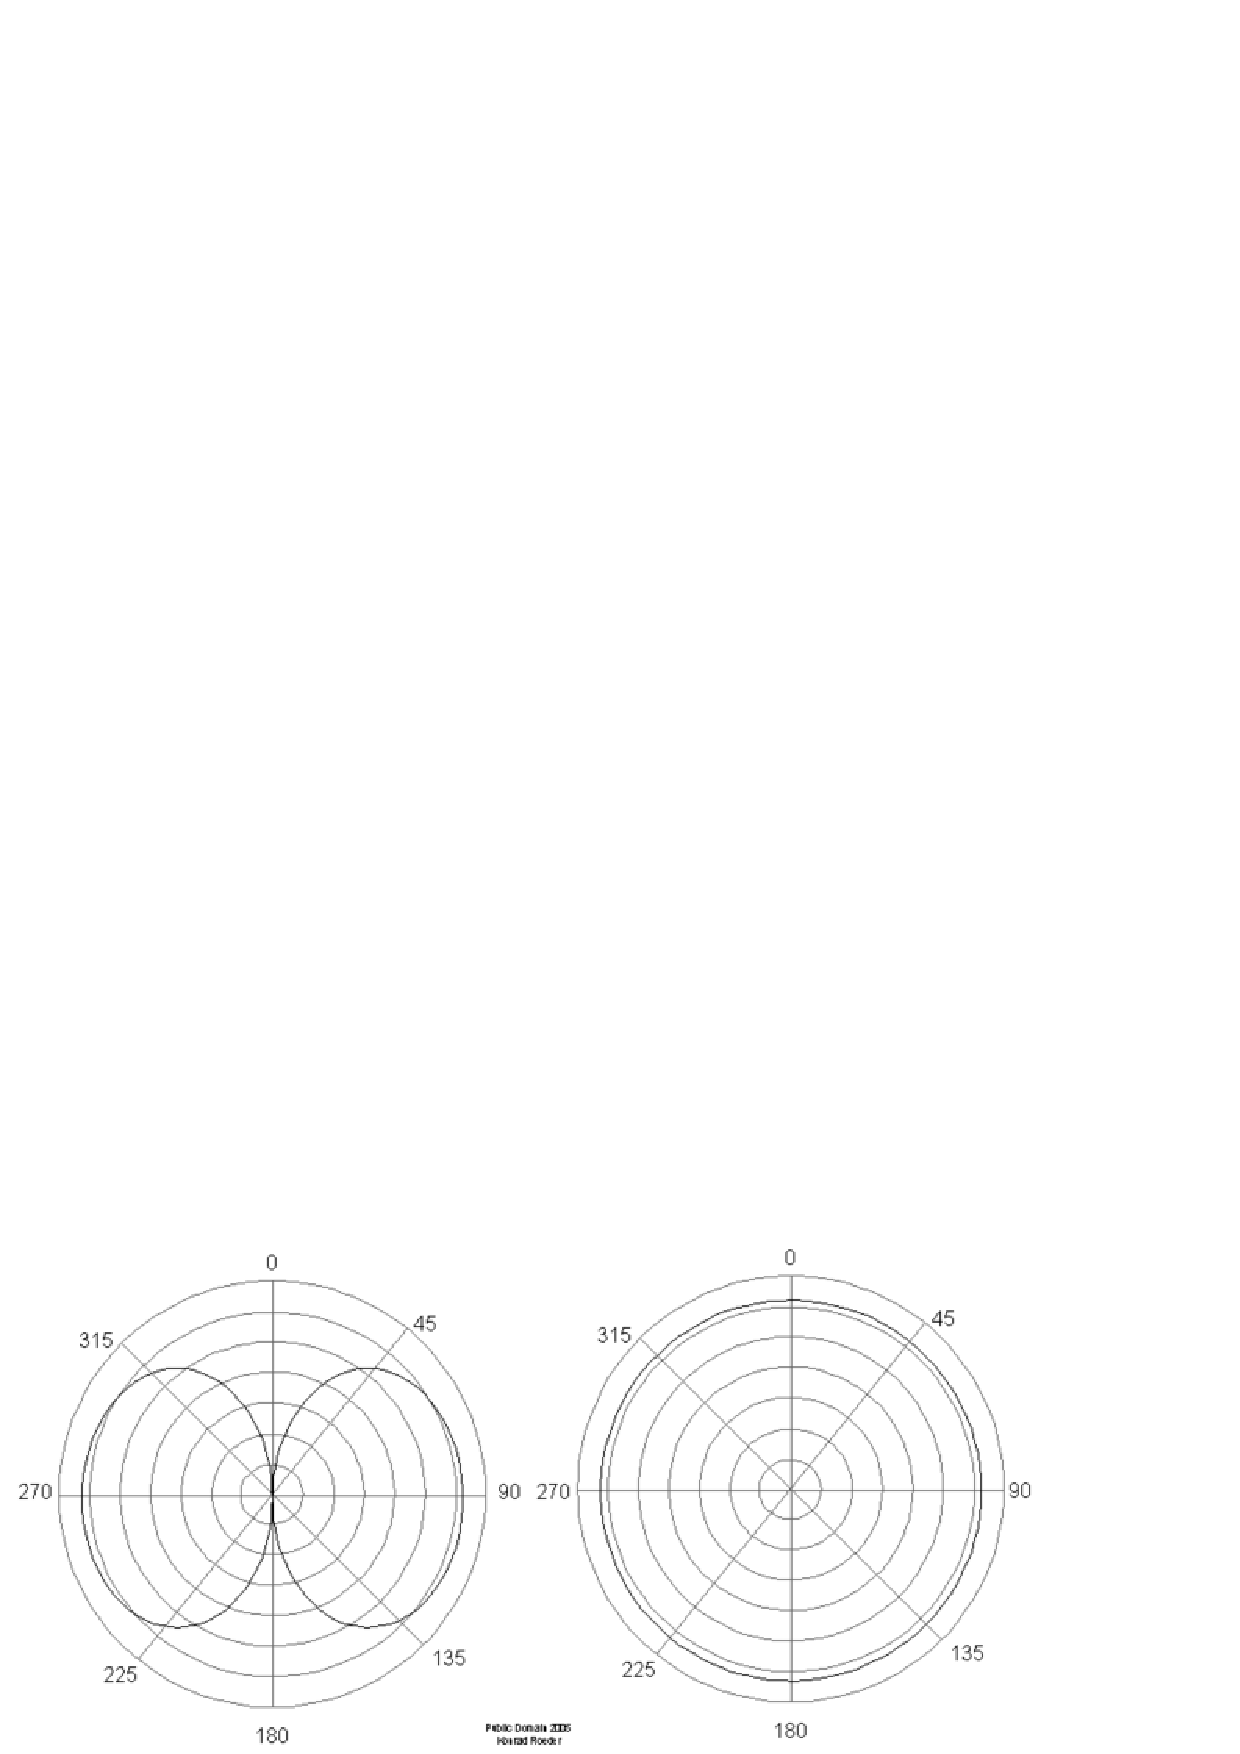
\includegraphics[width=\textwidth]{./Imagenes/06.01.adf/diagramas-radiacion.png}  
  \caption{Diagramas de radiaci\'on \cite{wikipedia_esp}}
  \label{fig:diagramas-radiacion}
\end{figure}

\end{description}


\subsection{Modulaci\'on}

Cuando se compara el rango de frecuencia t\'ipico de la voz humana (400 Hz a 4000 Hz) con el rango de frecuencia de las ondas de radio (a partir de los 30 kHz, aproximadamente), se hace evidente que no es posible convertir directamente de sonido a radio. Es necesario llevar a cabo un proceso intermedio para transmitir una onda de baja frecuencia utilizando una de mayor frecuencia.

Se define entonces la Modulaci\'on como el proceso de alterar las caracter\'isticas de una onda (llamada portadora o carrier) para que transporte informaci\'on.

Son varios los par\'ametros de la portadora que se pueden alterar, pero los m\'as habituales en el contexto aeron\'autico son la amplitud y la frecuencia.

\begin{description}

\item [AM] Se modifica la amplitud de la portadora en proporci\'on directa a la se\~nal moduladora. Este fue el primer m\'etodo para la emisi\'on de radio comercial. En la Figura \ref{fig:modulacion-am} se esquematiza la modulaci\'on AM.


\item [FM]La informaci\'on se representa mediante variaciones de la frecuencia instant\'anea de la onda portadora.
La modulaci\'on FM se representa en la Figura \ref{fig:modulacion-fm}.

  \begin{figure}[!h]
    \centering
\subfigure[Modulaci\'on en amplitud \cite{wikipedia_esp}]{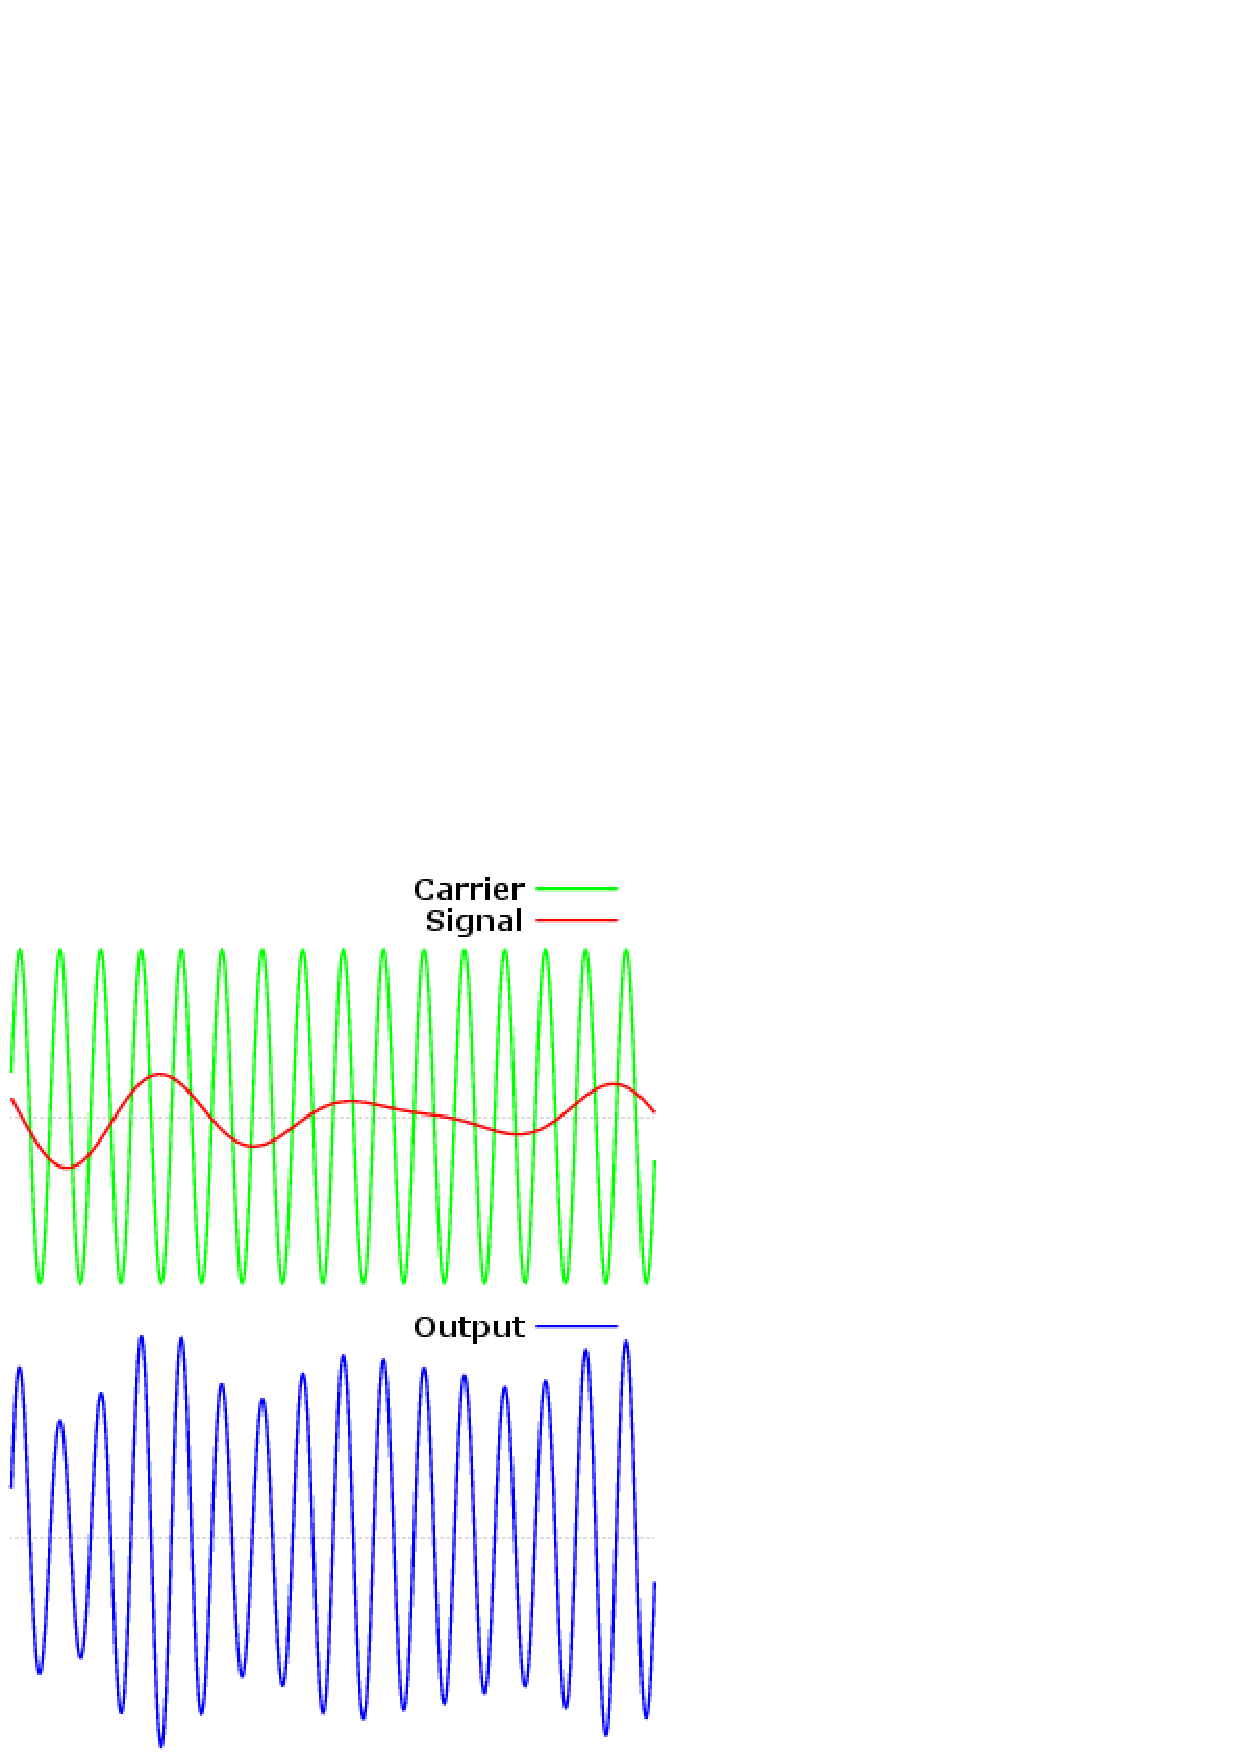
\includegraphics[width=0.45\textwidth]{./Imagenes/06.01.adf/modulacion-am.png} \label{fig:modulacion-am}}
\subfigure[Modulaci\'on en frecuencia \cite{wikipedia_esp}]{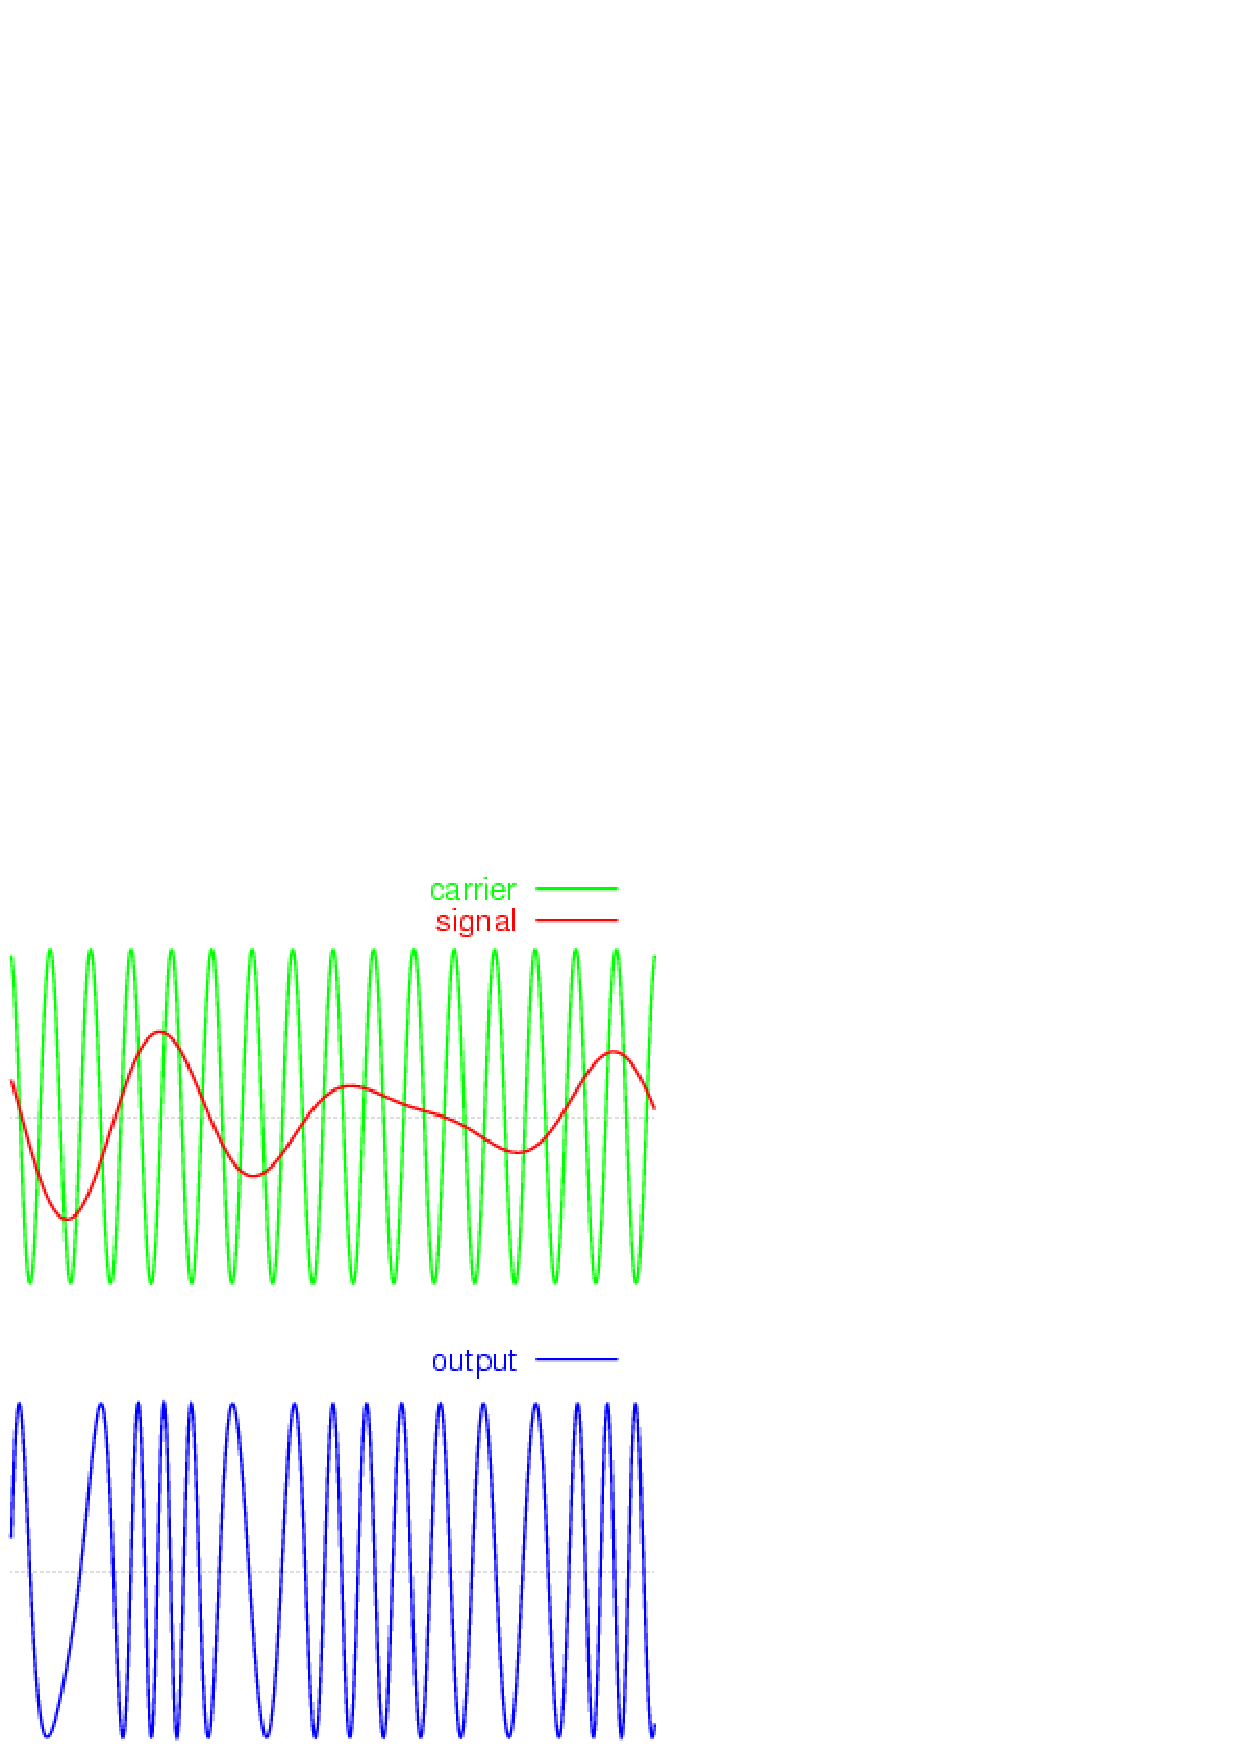
\includegraphics[width=0.45\textwidth]{./Imagenes/06.01.adf/modulacion-fm.png} \label{fig:modulacion-fm}}
\caption{Modulaci\'on de ondas electromagn\'eticas}
  \end{figure}


\item [Bandas laterales] En comunicaciones v\'ia radio se denomina as\'i a las bandas de frecuencias su\-pe\-rio\-res y/o inferiores a la de la portadora que aparecen por causa del proceso de modulaci\'on.


\item [Canal] Es una banda de radiofrecuencia espec\'ifica que ha sido asignada para un uso dado por medio de acuerdos internacionales. Por ejemplo, los canales de voz en aeron\'autica tienen un ancho predefinido de 50 kHz, lo que incluye el espacio para la banda de voz, las bandas laterales que aparezcan al modular, y unos margenes en los extremos para separarlos adecuadamente de los canales adyacentes.  



\end{description}

\subsection{El espectro electromagn\'etico}

Se denomina espectro electromagn\'etico a todo el rango posible de radiaci\'on electromagn\'etica. Esto incluye las ondas de radio, los infrarrojos, la luz, los ultravioletas, los rayos X, gamma, etc.
  En la Figura \ref{fig:espectro-electromagnetico} se presenta el espectro completo.

\begin{figure}[!h]
  \centering
 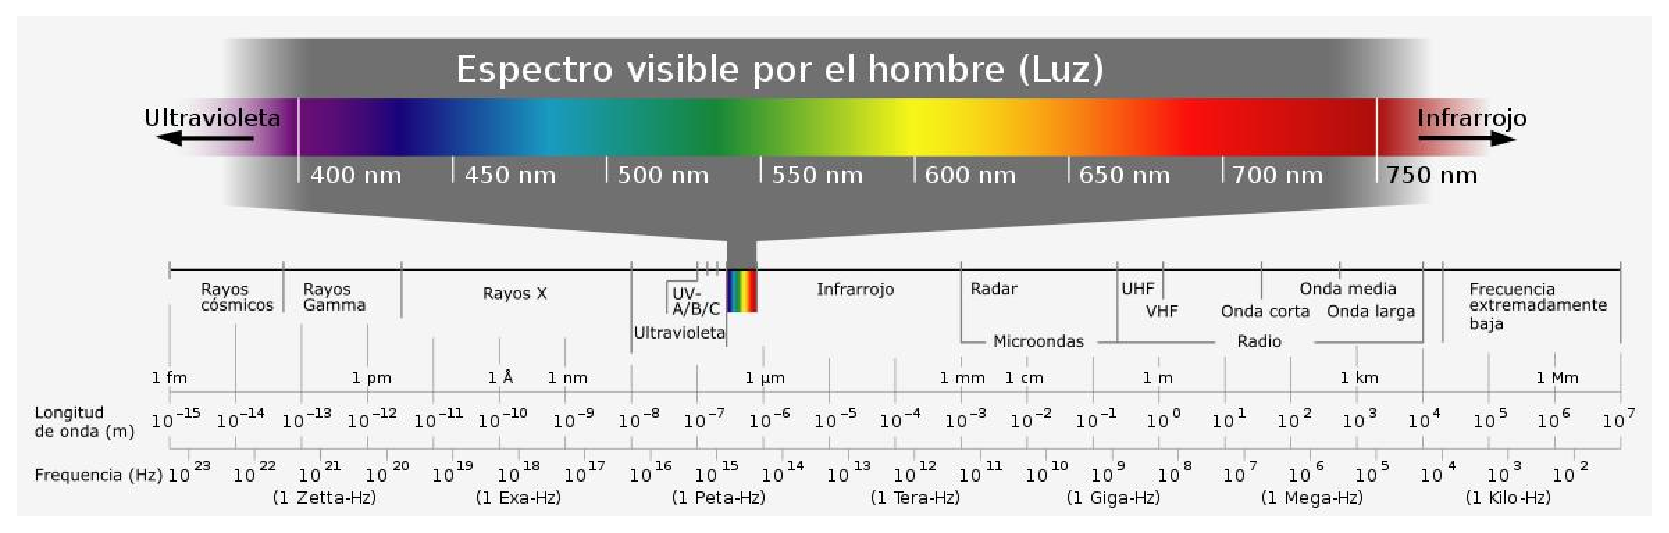
\includegraphics[width=\textwidth]{./Imagenes/06.01.adf/electromagneticspectrumes.eps}   
  \caption{Espectro electromagn\'etico}
  \label{fig:espectro-electromagnetico}
\end{figure}

En funci\'on de lo anterior, el espectro radioel\'ectrico o de radiofrecuencia (RF) se refiere a la porci\'on del espectro electromagn\'etico en el cual las ondas electromagn\'eticas pueden generarse alimentando a una antena con corriente alterna. La Tabla \ref{tab:espectro-radioelectrico}   presenta las bandas de RF m\'as importantes. 

\begin{table}[!h]
  \centering 
\label{tab:espectro-radioelectrico}
\caption{ Espectro radioel\'ectrico}
  \begin{tabular}{|c|l|c|c|}
 \hline \rowcolor{yellow!30}
{\bf Abreviatura} & \multicolumn{1}{c}{\bf  Nombre}
& {\bf Frecuencia} & {\bf Algunos usos}\\ \hline \hline
VLF 	& Very Low Frequency& 	3-30 kHz &	Loran-C \\ \hline
LF 	&Low Frequency 	&30-300 kHz &	ADF/NDB \\ \hline
MF 	&Medium Frequency 	&300-3000 kHz 	&ADF/NDB \\ \hline
HF 	&High Frequency 	&3-30 MHz 	&COMM larga distancia \\ \hline
VHF 	&Very High Frequency 	&30-300 MHz 	&VOR, COMM ACFT \\ \hline
UHF 	&Ultra High Frequency 	&300-3000 MHz 	&DME, radar, GNSS \\ \hline
SHF 	&Super High Frequency 	&3-30 GHz 	&Radar, COMM microondas \\ \hline
EHF 	&Extremely High Frequency &30-300 GHz 	&Radioastronom\'ia \\ \hline
\end{tabular}  
%\label{tab:espectro-radioelectrico}
\end{table}

A mayor frecuencia la longitud de onda se reduce, raz\'on por la cual es posible encontrar tambi\'en la tabla anterior en funci\'on de la longitud y clasificando el espectro en ondas kilom\'etricas, decim\'etricas, milim\'etricas, etc.  	  	 

\subsection{Propiedades de la propagaci\'on}

Las caracter\'isticas de la propagaci\'on de las ondas electromagn\'eticas son importantes para comprender algunas de las caracter\'isticas de los sistemas que las utilizan. Por eso, en esta secci\'on se repasar\'an los aspectos m\'as importantes de la propagaci\'on.

Hay algunas propiedades generales de la propagaci\'on que son independientes de la frecuencia de la onda RF de la cual se est\'e hablando:

\begin{itemize}

\item  La velocidad de una onda electromagn\'etica es constante mientras no
  cambie el medio de propagaci\'on.

  \item La velocidad de una onda electromagn\'etica en el vac\'io es siempre $c
  = 299792458 \,\text{m/s}$.

  \item Las ondas electromagn\'eticas tienden a reflejarse en objetos de
  tama\~no similar a su longitud de onda ($\lambda$).

  \item Las ondas electromagn\'eticas se propagan en l\'inea recta mientras no
  sufran influencias externas ni cambien de medio de propagaci\'on
\end{itemize}
.

Es oportuno recordar que la reflexi\'on es el cambio abrupto en la direcci\'on de la onda cuando \'esta llega a la uni\'on de dos medios diferentes, regresando al medio original (Figura \ref{fig:reflection-ondas}) . 

Por otro lado, la refracci\'on es el cambio en velocidad de una onda cuando pasa de un medio a otro. Es de hacer notar que a menudo el cambio en velocidad implica un cambio de direcci\'on (dado que la velocidad es un vector), tal como se muestra en la Figura \ref{fig:refraccion-ondas}.

\begin{figure}[!h]
  \centering
  \subfigure[Fen\'omeno de reflecci\'on \cite{wikipedia_esp}]{\includegraphics[height=7cm]{./Imagenes/06.01.adf/Imagenes/Reflection_angles-eps-converted-to.pdf}\label{fig:reflection-ondas}}
  \subfigure[Fen\'omeno de refracci\'on \cite{wikipedia_esp}]{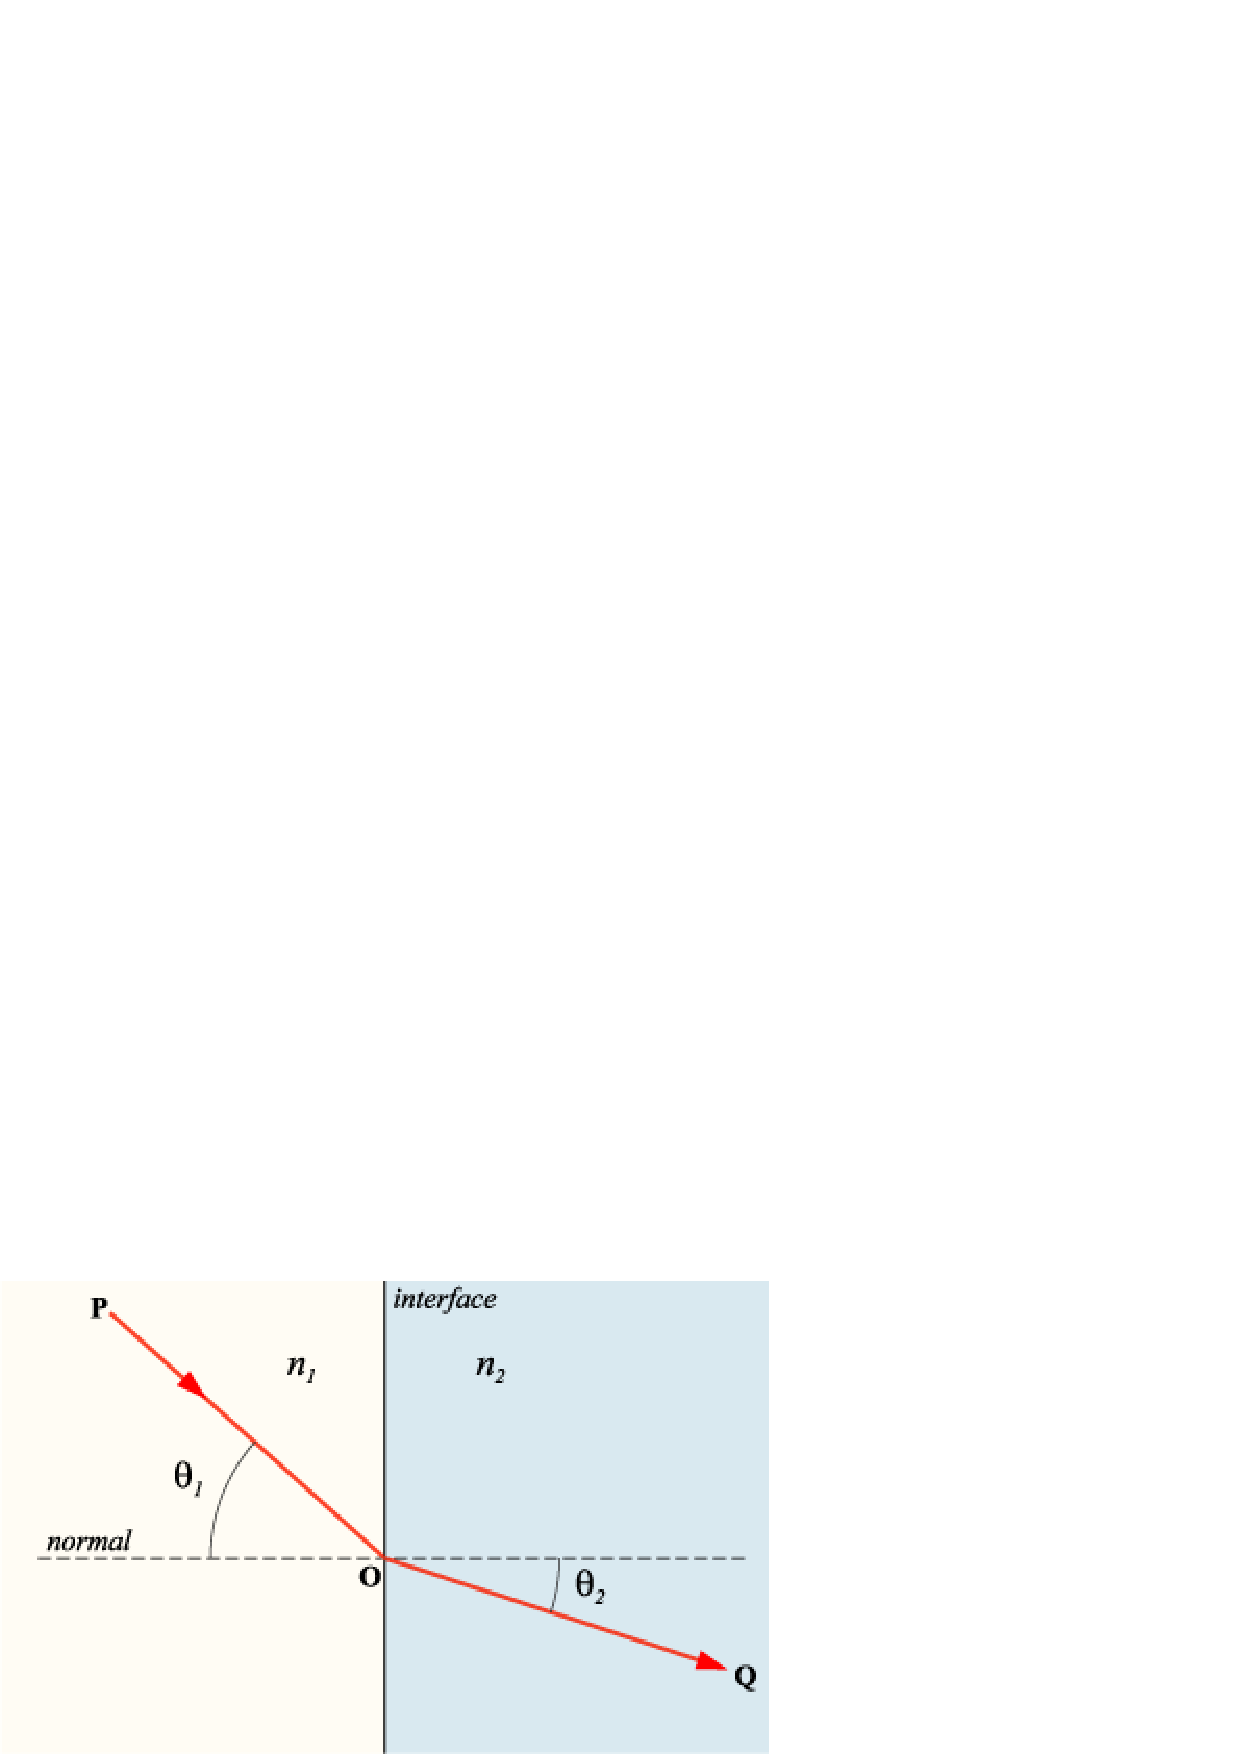
\includegraphics[height=7cm]{./Imagenes/06.01.adf/refraccion-ondas.png}\label{fig:refraccion-ondas}}
  \caption{Fenomenos que ocurren en la propagaci\'on de las ondas}
\end{figure}

Un concepto estrechamente relacionado con el de la refracci\'on es el del \'angulo l\'imite o \'angulo cr\'itico. Cuando el \'angulo de incidencia de la onda con respecto a la normal es mayor que dicho \'angulo, la onda se refleja en vez de refractarse.

La expresi\'on para el \'angulo l\'imite es la  $ \theta_{crit} = \arcsin(n_2/n_1) $, donde $n_1$ y $n_2$ son los \'indices de refracci\'on de los medios de origen y destino, respectivamente.

Finalmente, pero no por ello menos importante, hay que tener en cuenta que la potencia de una onda electromagn\'etica va disminuyendo mientras se aleja de la fuente con una relaci\'on inversamente proporcional al cuadrado de la distancia.

\begin{figure}[!h]
  \centering
  \includegraphics[width=0.95\textwidth]{./Imagenes/06.01.adf/propagacion-ondas.gif}
  \caption{Propagaci\'on de ondas}
  \label{fig:propagacion.de.ondas}
\end{figure}

Por otro lado, hay propiedades de la propagaci\'on que son fuertemente dependientes de la frecuencia de la onda. Si bien no hay una separaci\'on estricta entre cada caso, se suele dividir a las ondas en tres grandes tipos seg\'un su forma predominante de propagaci\'on: 


\begin{description}
  \item[Ondas de tierra (Surface Waves)] Tambi\'en denominadas ondas de suelo se caracterizan porque aprovechan las propiedades conductivas del terreno (tierra, agua, etc.) para propagarse, siempre que la frecuencia de emisi\'on se encuentre debajo de los 5 Mhz. De esta manera, son capaces de sortear grandes obst\'aculos y llegar muy lejos, \textcolor{blue}{\bf con un alcance casi global}. A pesar de su nombre, no es necesario estar en el suelo para poder recibirlas.
Se emplea en las mismas polarizaci\'on vertical para reducir su atenuaci\'on al ponerse en contacto con la tierra, Figuras \ref{fig:propagacion.de.ondas} y \ref{fig:ondas.de.tierra}.

Este tipo de propagaci\'on es predominante en las frecuencias bajas (VLF, LF y MF, principalmente, $\approx 3$ MHz), y por ello se requiere de grandes antenas y mucha potencia para emitirlas y recibirlas.

\begin{figure}[!h]
  \centering
  \subfigure[Ondas de tierra]{
	\includegraphics[height=4.5cm]{./Imagenes/06.01.adf/surface-waves-gif-converted-to.png}
	  \label{fig:ondas.de.tierra}
	}
  \subfigure[Ondas de l\'inea de vista]{
	\includegraphics[height=4.5cm]{./Imagenes/06.01.adf/space-wave-gif-converted-to.png}
	  \label{fig:space.waves}
	}
  \caption{Propagaci\'on de ondas}
\end{figure}

El hecho de que su alcance sea tan grande limita su uso, pues plantea el problema de potenciales interferencias entre estaciones muy lejanas. Asimismo, su trayectoria puede ser dif\'icil de predecir dado que se refractan en las fronteras entre medios diferentes, como por ejemplo las costas (tierra/agua). 

Tambi\'en suelen emplearse para comunicaciones a distancias cortas con un rango de frecuencias entre 3-30 MHz.

El Loran-C es una de las pocas radioayudas que utiliza este tipo de ondas. 


\item[Ondas ionosf\'ericas  u ondas de cielo (Skyline Waves)] Aprovechan las caracter\'isticas el\'ectricas de la ionosfera para propagarse, us\'andola como una especie de ``espejo''. En realidad, m\'as que una reflexi\'on es una refracci\'on progresiva limitada por el \'angulo cr\'itico (lo que implica que cierta cantidad de energ\'ia se escapa al espacio). Es predominante en las frecuencias medias: MF y HF.

Evidentemente, una propagaci\'on de este tipo se ve fuertemente influenciada por la geometr\'ia relativa entre emisor, ionosfera y receptor. Para complicar la situaci\'on, la posici\'on y caracter\'isticas de la ionosfera son altamente variables, pues dependen del Sol. Por eso, la situaci\'on es diferente durante el d\'ia y durante la noche, y cambia seg\'un la estaci\'on del a\~no y el ciclo solar. Adicionalmente, el terminator line\footnote{Se puede entender mejor este concepto mediante el simulador Earth Viewer \url{http://www.paulcarlisle.net/old/earthviewer.html} } (frontera entre el d\'ia y la noche) tambi\'en afecta la propagaci\'on,  Figuras \ref{fig:propagacion.de.ondas}.

Debido a esta compleja situaci\'on aparecen ``zonas de oscuridad'', es decir, zonas donde no hay recepci\'on porque ninguna onda ha rebotado con la geometr\'ia adecuada para proporcionar cobertura. Asimismo, es posible que hayan m\'ultiples rebotes sucesivos (proporcionando un alcance muy largo pero inestable).

Otro problema que presentan estas ondas es el efecto fadding: a cierta distancia del emisor, el receptor puede recibir la misma onda pero que ha seguido caminos diferentes (una parte se propag\'o como onda de tierra y otra como de cielo), ocasionando interferencia destructiva y resultando en una se\~nal que aparece y desaparece r\'apidamente.

En el \'ambito aeron\'autico, el ADF/NDB y las comunicaciones de largo/medio alcance utilizan este tipo de propagaci\'on. 


\item[Ondas de l\'inea de vista (Space Waves)] Se propagan en l\'inea recta, de forma an\'aloga a como lo har\'ia la bala de un rifle. Debido a lo anterior, su alcance es limitado y no pueden rodear obst\'aculos de tama\~no medio, Figuras \ref{fig:propagacion.de.ondas} y \ref{fig:space.waves}.

Esta limitaci\'on se convierte en una ventaja dado que entonces es posible reutilizar las frecuencias una y otra vez si los emisores/receptores est\'an lo suficientemente alejados entre s\'i. Adem\'as, las frecuencias altas (VHF y superior) en donde este tipo de propagaci\'on predomina son mucho menos suceptibles a la interferencia por causa de est\'aticos.

Debido a sus ventajas, la inmensa mayor\'ia de las comunicaciones y aplicaciones aeron\'auticas modernas (VOR, DME, ILS, GNSS y un largo etc\'etera) se hace con ondas de l\'inea de vista.

\end{description}

\section{Sistema de Navegaci\'on Hiperb\'olicos}

\subsection{Introducci\'on}

Los Sistemas de Navegaci\'on Hiperb\'olicos son aquellos que utilizan como t\'ecnica de localizaci\'on de la aeronave la intersecci\'on de hip\'erbolas. Son sistemas de largo alcance, utilizados en vuelos intercontinentales o transoce\'anicos.

\begin{figure}[!h]
  \centering
\includegraphics[width=0.7\textwidth]{Imagenes/06.01.adf/Hiperbola.gif}
  \caption{Elementos de una hip\'erbola}
  \label{fig:hiperbola}
  \label{!h}
\end{figure}


La hip\'erbola es una de las c\'onicas (elipse, par\'abola, hip\'erbola) y se define como el lugar geom\'etrico de los puntos cuyas diferencias de distancias a dos puntos fijos, denominados focos, es constante. Matem\'aticamente esto se expresa como:

\[\mathbf{FP}-\mathbf{F'P}= 2a
\]

Donde los puntos $F$ y $F'$ son los focos de la c\'onica (Figura \ref{fig:hiperbola}), y $2a$ es la distancia entre los dos v\'ertices de las curvas.

El principio de funcionamiento de los sistemas hiperb\'olicos se basa en que la aeronave tenga a borde el equipo necesario para determinar la diferencia de distancias que la separan de dos estaciones fijas situadas en tierra. Para ello se asume que las dos estaciones terrestres, ubicadas en los focos, emiten ondas electromagn\'eticas en todas direcciones. El punto $P$ que representa a la aeronave, recibe las ondas y determina la diferencia de distancias que la separan de las estaciones terrestres.

De esta manera, el operador a bordo de la aeronave, determina en que ``hip\'erbola'' se encuentra, pero no sabe en que punto de la misma est\'a ubicado. 
Para solucionar esto se requiere una hip\'erbola m\'as, lo que se logra
con un sistema de tres estaciones terrestres, 
a fin de minimizar la indeterminaci\'on a dos posibles puntos 
o tres hip\'erbolas para localizar la nave en un \'unico punto. 
Con dos curvas sobra precisi\'on para la localizaci\'on ya que, 
de los dos puntos posibles, uno se desestima por encontrarse muy alejado de la ruta.

Han existido diversos sistemas de navegaci\'on hiperb\'olicos, pero la mayor\'ia no operan actualmente o han sufrido modificaciones. Entre ellos se tiene:
\begin{multicols}{2}
\begin{itemize}
\item GEE

\item LORAN-A
\item  LORAN-B
\item LORAN-C
\item LORAN-D

\item DECCA

\item OMEGA

\item TROPIK

\item MARSHRUT

\item SHORAN (SHOrt Range Air Navigation)
\end{itemize}
\end{multicols}

\begin{figure}[!h]
  \centering
  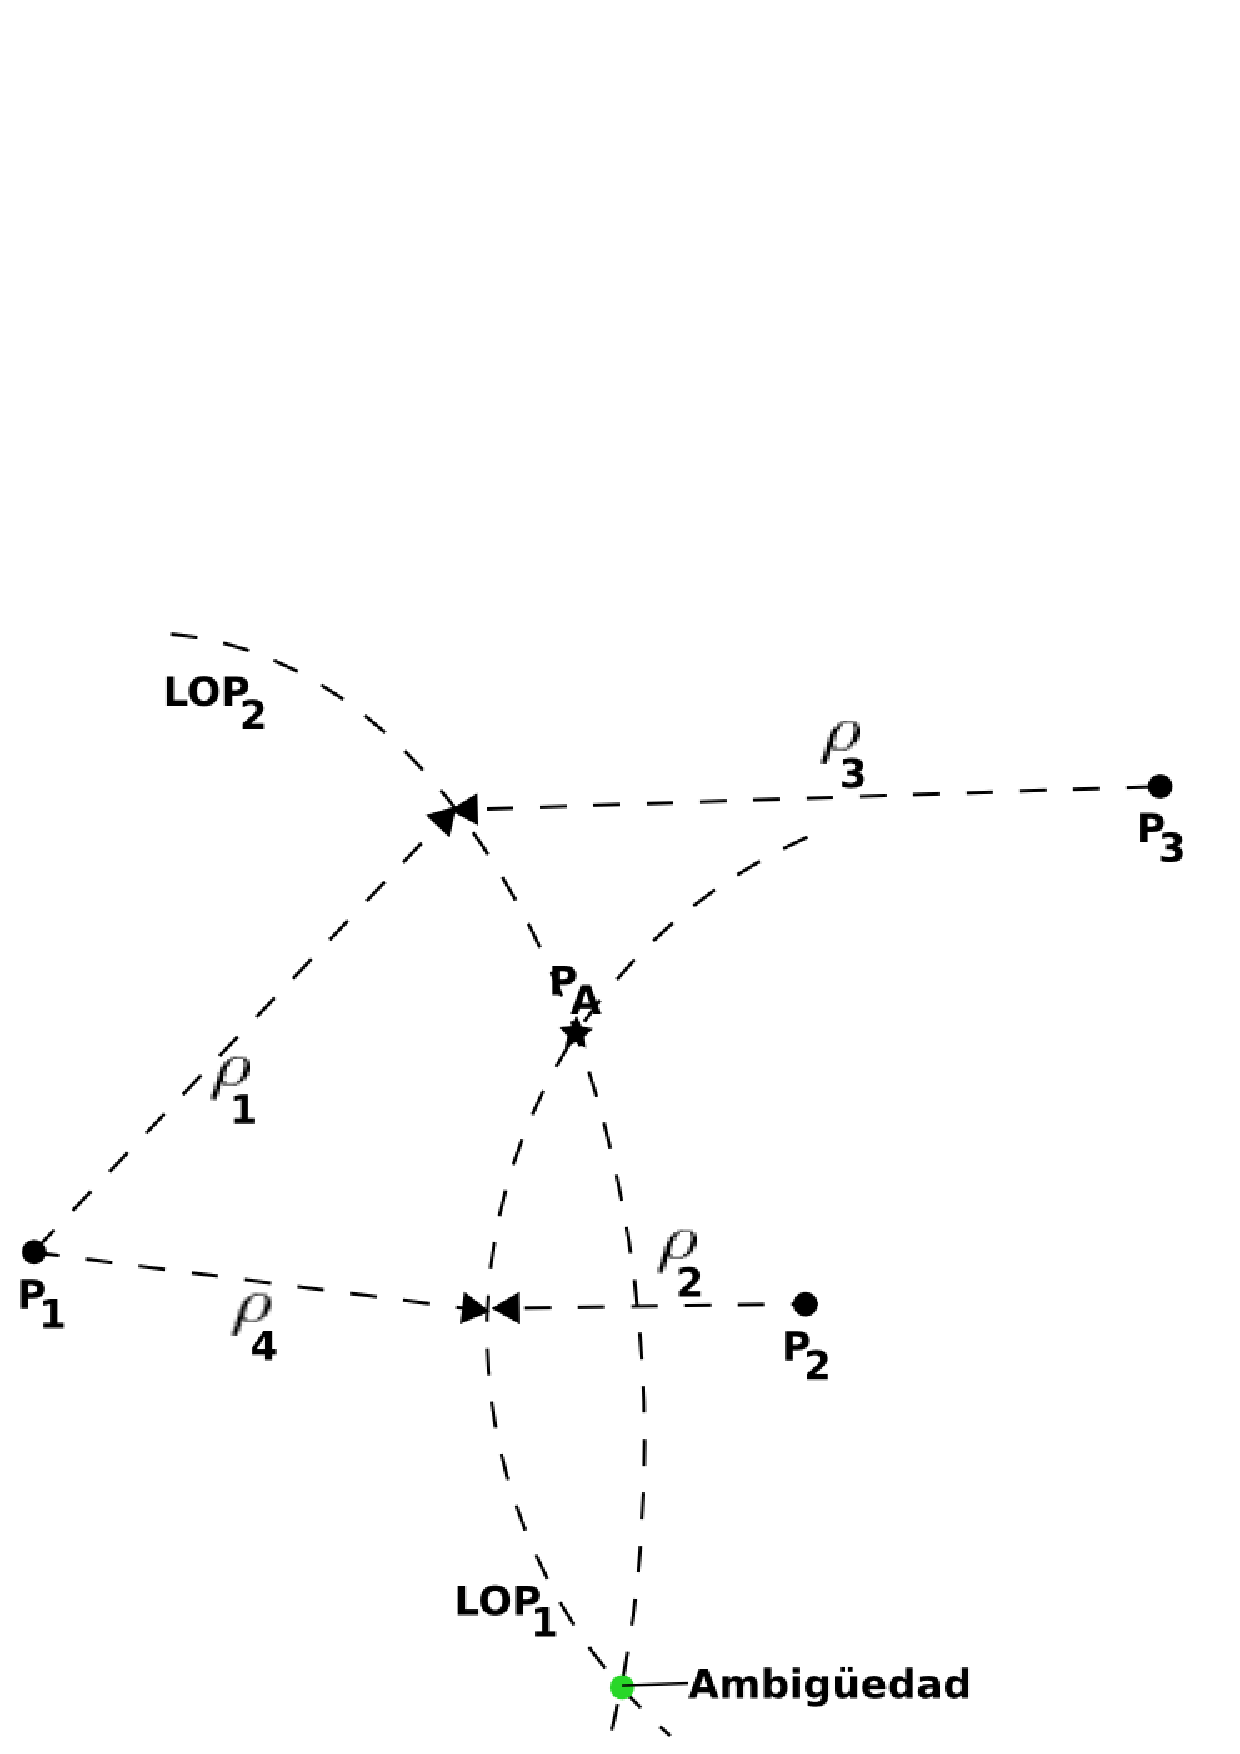
\includegraphics[width=0.5\textwidth]{Imagenes/06.01.adf/hiperbolic-fix.png}
  \caption{Principio de ubicaci\'on de la posici\'on por navegaci\'on hiperb\'olica}
  \label{fig:principio.navegacion.hiperbolica}
\end{figure}


\subsubsection{T\'ecnicas de navegaci\'on hiperb\'olica}

Los sistemas hiperb\'olicos solo pueden determinar diferencias de distancias, para ello se emplean dos t\'ecnicas diferentes:

\begin{description}
\item [T\'ecnica de impulsos-tiempos:] conociendo la velocidad de las ondas electromagn\'eticas, $\mathbf{c}$, se puede relacionar el tiempo medido con la distancia recorrida mediante la expresi\'on:

\[ \Delta\,r = c\,\Delta t
\]

De donde:

\[ r = r_0+c\,\left(t-t_0\right)
\]

\begin{wrapfigure}{right}{0.4\textwidth}
  \input{Imagenes/06.01.adf/triangulo-situacion.tex}
\end{wrapfigure}

Pero la ecuaci\'on encierra una gran dificultad de llevar a la pr\'actica puesto que $t_0$ implica conocer el momento exacto en que se produjo la transmisi\'on del emisor. Este problema desaparece si se considera, en lugar de una distancia determinada a una estaci\'on, una diferencia de distancias a dos estaciones puesto que si ambas transmiten sincronizadas, al efectuarse la diferencia de distancia la inc\'onita $t_0$ desaparece.

Para ver con mas detalle lo anterior, consid\'erese una estaci\'on emisora maestra, $M$  que empieza su emisi\'on en el tiempo $t_0$; otra estaci\'on denominada esclava ubicada a una distancia $d$ de la estaci\'on maestra, recibe esta se\~nal luego de un tiempo $d/c$. Luego de un tiempo $\tau$, denominado ``tiempo de sincronismo'', emite una se\~nal id\'entica a la recibida. 

El receptor en la aeronave ($A$) recibe las se\~nales emitidas por las emisoras maestra y esclava, calculando la diferencia de tiempo entre ambas $\Delta\,t = t_2-t_1$. 

Partiendo de la estaci\'on maestra en el tiempo $t_0$, el impulso tarda un tiempo $t_1-t_0$ en llegar al receptor de la aeronave:

\[t_1-t_0 = \displaystyle \frac{r_1}{c}
\]

Al llegar el impulso de la estaci\'on madre a la esclava, esta luego del tiempo $\tau$, emite el suyo el cual llega en el tiempo $t_2$ al receptor, de esta forma se tiene:

\[
t_2-t_0 = \displaystyle \frac{d}{c}+\tau+\frac{r_2}{c}
\]

Haciendo la diferencia de $t_2-t_1$ seg\'un las expresiones anteriores:

\[
t_2-t_1 = t_0 + \displaystyle \frac{d}{c}+\tau+\frac{r_2}{c} - t_0 -\frac{r_1}{c} = \tau+\frac{d+r_2-r_1}{c} = \tau+\frac{d+\Delta\,r}{c}
\]

Finalmente:

\[
\Delta\,t = \tau+\frac{d+\Delta\,r}{c}
\]

Esta expresi\'on implica que a cada incremento de tiempo ($\Delta t$) le corresponde uno de distancia ($\Delta r$), con los par\'ametros $d$, $c$ y $\tau$ conocidos.

Pero debe recordarse algo, en lugar de considerar hip\'erbolas que son curvas planas, este m\'etodo ubica al receptor en un hiperboloide de revoluci\'on. Por esto deben hacerse correcciones por la curvatura y forma de la tierra.


\item [T\'ecnica de onda continua-fases:]

En esta t\'ecnica la emisi\'on es de forma continua a diferencia de la anterior que es por pulsos y que el par\'ametro que se mide es la diferencia de fases.

Se utilizan dos emisores omnidireccionales con un sincronismo de fases entre sus se\~nales. El receptor recibe a ambas se\~nales con una diferencia de fase, que depende de la distancia de la aeronave a cada una de las emisoras. De esta manera se determina la hip\'erbola donde se encuentra el receptor.

Conociendo la longitud de onda $\lambda$ se puede obtener la distancia recorrida seg\'un la fase medida: 

\[\Delta r = \lambda \,\Delta \phi \quad \Longrightarrow r = r_0 +\lambda \,\left( \phi - \phi_0 \right) \]

Aqui se presenta una dificultad porque el receptor necesita conocer $ \phi_0$, la fase exacta en que se produjo la transmisi\'on.

El proceso se realiza de la siguiente forma, la estaci\'on maestra ubicada en $M$ emite su se\~nal continua con frecuencia $f_1$ (longitud de onda $\lambda_1$) y origen de fases $ {\phi_1}_0$. La estaci\'on esclava en $E$ recibe esta se\~nal y transmite la suya con frecuencia $f_2$ y fase inicial $ {\phi_2}_0$. La frecuencia $f_2$ es diferente de la $f_1$ para que el receptor pueda separar facilmente las se\~nales.

La antena de la aeronave recibe ambas se\~nales $f_1$ y $f_2$ con fases $\phi_1$ y $\phi_2$ diferentes a las de salida, cuyos valores son:

\[
\phi_1 = {\phi_1}_0 + \displaystyle \frac{r_1}{\lambda_1} \qquad
\phi_2 = {\phi_2}_0 + \displaystyle \frac{r_2}{\lambda_2} 
\]

Para poder comparar estas se\~nales se usa el artificio de una frecuencia com\'un, $f_c$, con longitud de onda $\lambda_c$ que resulta de multiplicar a cada una de las frecuencias anteriores por un n\'umero entero $n_1$ y $n_2$, respectivamente:

\[
f_c = n_1\,f_1 = n_2\,f_2
\]

Cuando se multiplica una frecuencia por un n\'umero, se hace lo mismo con su fase, por lo que las expresiones anteriores vistas desde esta frecuencia com\'un, quedan:

\[
\theta_1 = n_1\,\phi_1 = n_1\,{\phi_1}_0 + \displaystyle \frac{n_1\,r_1}{\lambda_1} \qquad
\theta_2 = n_2\,\phi_2 = n_2\,{\phi_2}_0 + \displaystyle \frac{n_2\,r_2}{\lambda_2} 
\]

Restando la diferencia de las fases:

\[
\Delta\,\theta = \theta_1-\theta_2 = n_1\,{\phi_1}_0 + \displaystyle \frac{n_1\,r_1}{\lambda_1} -  n_2\,{\phi_2}_0 - \displaystyle \frac{n_2\,r_2}{\lambda_2} 
\]

El sincronismo de fase entre la estaci\'on maestra y la esclava debe realizarse de forma que se cumpla lo siguiente:

\begin{itemize}
\item La diferencia de fases iniciales multiplicadas por su entero respectivo debe mantenerse constante: $n_1\,{\phi_1}_0- n_2\,{\phi_2}_0= cte$

\item El ajuste de sincronismo que realiza la estaci\'on esclava cumple, en la prolongaci\'on de la l\'inea que la une con la maestra pero en el lado de la maestra, que la diferencia de fases en la aeronave sea nula: 

Para $r_1=0$ y $r_2=d$ se cumple que $\Delta\,\theta = \theta_1-\theta_2 =0$

\end{itemize}

Sabiendo que para un lado se cumple $c = f_c\,\lambda_c = f_1\,\lambda_1$ y como $f_c=n_1\,f_1$, entonces $n_1f_1\lambda_c = f_1\lambda_1$, por lo que $n_1\lambda_c=\lambda_1$ o $\displaystyle \frac{n_1}{\lambda_1}=\frac{1}{\lambda_c}$.

De la misma manera se obtiene $\displaystyle \frac{n_2}{\lambda_2}=\frac{1}{\lambda_c}$.

Volviendo a la diferencia de fases de la frecuencia com\'un:

\[
\Delta\,\theta = n_1\,{\phi_1}_0- n_2\,{\phi_2}_0 +  \displaystyle \frac{n_1\,r_1}{\lambda_1}  - \displaystyle \frac{n_2\,r_2}{\lambda_2}= cte + \frac{\Delta r}{\lambda_c}
\]

Trabajando con la expresi\'on anterior se llega a que:

\[
\Delta \theta = \displaystyle \frac{d+\Delta r}{\lambda_c}
\]

Surge un problema adicional, esta expresi\'on solo resuelve el incremento de fase dentro de una longitud de onda determinada pero se desconoce dentro de cual. 
Esto resulta en una indeterminaci\'on m\'ultiple, ya que el \'angulo real ser\'a un n\'umero entero de longitudes de onda m\'as el desfase obtenido de la ecuaci\'on anterior. 
La indeterminaci\'on ser\'a mayor cuanto mayor sea la frecuencia de la se\~nal radiada (menor $\lambda$). 
El inconveniente se soluciona con otra t\'ecnica conocida como del n\'umero de longitudes de onda completas.


\end{description}


\subsection{LORAN}


El \textbf{LORAN} (del ingl\'es LOng RAnge Navigation, navegaci\'on de largo alcance) es un sistema de ayuda a la navegaci\'on electr\'onica de tipo hiperb\'olico
 de largo alcance, que opera en baja y media frecuencia. 

Utiliza el intervalo transcurrido entre la recepci\'on de se\~nales de radio transmitidas desde tres o m\'as transmisores para determinar la posici\'on del receptor. 

Desarrollado a principios de la II Guerra Mundial, el LORAN fue el primer sistema de navegaci\'on basado en la llegada diferenciada de se\~nales de radio. Fue concebido por el laboratorio de Radiaci\'on de MIT. LORAN fue, tambi\'en, el primer sistema de posicionamiento capaz de funcionar bajo cualquier condici\'on climatol\'ogica pero es solamente bidimensional (latitud y longitud).

\begin{figure}[!tbh]
  \centering
  \subfigure[Interior de la instalaci\'on emisora]{\includegraphics[height=5.5cm]{Imagenes/06.01.adf/LORAN-Equip-Hut_.jpg}}
  \subfigure[Vista de estaci\'on emisora]{\includegraphics[height=5.5cm]{Imagenes/06.01.adf/LORAN-A_1940-instalacion-terrestre.jpg}}
  \caption{Instalaciones de LORAN-A \cite{Historia_LORAN} }
\end{figure}

 El sistema emisor LORAN se compone de una estaci\'on maestra y otra esclava. La maestra emite de forma regular una peque\~na se\~nal, que es repetida por la esclava, controlada por radio desde la maestra. Ambas se\~nales se reciben en el barco o avi\'on, se amplifican y se registran como peque\~nas ondas sobre la pantalla de un tubo de rayos cat\'odicos. Los circuitos del receptor est\'an dispuestos de forma que la distancia entre las se\~nales corresponda a la diferencia de tiempos de llegada de las se\~nales de ambas estaciones. El receptor posee adem\'as un dispositivo temporizador electr\'onico que permite medir dicha diferencia en microsegundos (millon\'esimas de segundo).

Como las ondas de radio viajan a una velocidad aproximadamente constante de 300000 km/segundo, la ubicaci\'on de todos los puntos en los que las se\~nales de las dos estaciones est\'an separadas un determinado intervalo de tiempo se puede representar mediante una curva concreta que es una hip\'erbola (Figura \ref{fig:LORAN_hiperbolas}). El navegante dispone de un mapa con muchas de estas curvas, denominadas curvas de posici\'on LORAN, y tras determinar la diferencia de tiempos, por ejemplo, 3 microsegundos, sabe que la posici\'on de su nave se halla en alg\'un punto de la curva de 3 microsegundos del mapa. Sintonizando una pareja de emisores LORAN y repitiendo este proceso, el navegante es capaz de detectar otra curva que represente la posici\'on de la nave; la posici\'on real del aparato se halla en la intersecci\'on de las dos curvas LORAN. 


\begin{figure}[!tbh]
  \centering
  \includegraphics[width=0.95\textwidth]{Imagenes/06.01.adf/hypnavig.pdf}
  \caption{Mapa de hip\'erbolas del sistema LORAN \cite{Loran_conicas}}
  \label{fig:LORAN_hiperbolas}
\end{figure}


Este sistema posee un alcance \'util de unos 2592,8 km (1400 nm) por la noche y unos 1296,4 km (700 nm) de d\'ia. Las se\~nales se emiten generalmente en la banda de frecuencias de 1,8 a 2,0 MHz. Sirve tanto para marcar y mantener un rumbo, como para fijar la posici\'on, y presenta la ventaja de ser independiente de las condiciones meteorol\'ogicas. Su exactitud oscila entre unos centenares de metros y unos pocos kil\'ometros, dependiendo del equipo utilizado y de la distancia entre la nave y la emisora. 


La versi\'on m\'as moderna es LORAN-C que funciona en frecuencias del espectro electromagn\'etico entre 90 y 100 Khz. El sistema LORAN es utilizado en muchos pa\'ises, entre ellos los Estados Unidos de Am\'erica, Jap\'on y varios pa\'ises europeos. Rusia utiliza un sistema casi id\'entico llamado CHAYKA, que usa la misma banda de frecuencias. 

El uso de LORAN est\'a decayendo r\'apidamente siendo reeplazado por GPS. Sin embargo, se est\'a estudiando la posibilidad de mejorar y volver a popularizar el LORAN.

\begin{figure}[!tbh]
  \centering
    \includegraphics[width=\textwidth]{Imagenes/06.01.adf/Loran_A_Coverage_1973.jpg}
  \caption{Cobertura LORAN-A A\~no 1973 \cite{loran-history-info}}
  \label{fig:LORAN-A-cobertura-1973}
\end{figure}

\subsection{DECCA}

El sistema de navegaci\'on DECCA es un sistema hiperb\'olico de posicionamiento basado en se\~nales de radio de onda continua en el rango de frecuencias de los 70 a los 130 Khz. Su uso puede aplicarse tanto en entornos mar\'itimos, a\'ereos y terrestres. El sistema consta de estaciones emisoras en tierra situadas en localizaciones conocidas que crean l\'ineas de posici\'on hiperb\'olicas. El alcance del sistema depende de varios factores pero normalmente es del orden de 240 millas mar\'itimas (unos 440 Km) durante la noche y el doble de esta distancia por el d\'ia. Una cadena de estaciones DECCA consta de una estaci\'on central Master, a la que se asocian las tareas de supervisi\'on, control y monitorizaci\'on de la cadena, junto con tres, en algunos casos dos, estaciones esclavas alejadas a unos 80-110 Km. de la Master.

Inventado en Am\'erica por Wiilian J.O'Brien, pero desarrollado por la empresa londinense ``DECCA Radio and Televisi\'on, Ltd.'',el sistema DECCA se us\'o inicialmente para dirigir el rumbo de los dragaminas durante el desembarco de Normand\'ia en la Segunda Guerra Mundial. El DECCA comenz\'o a transmitir el 5 de junio de 1944. En 1975, Mr H. Schwarz, el director general de la Compa\~nia DECCA Navigator, admiti\'o que el Loran-C era probablemente mejor que el DECCA en navegaci\'on a\'erea y que la navegaci\'on por sat\'elite era posiblemente mejor que ambos. Ante la competencia del sistema GPS, DECCA suspendi\'o su servicio entre los a\~nos 2000 y 2001.\cite{wikipedia_esp}

\subsubsection{ Funcionamiento}


Para poder determinar exactamente la posici\'on de un m\'ovil en el espacio el Sistema DECCA necesita usar al menos tres estaciones transmisoras en tierra. Este conjunto de estaciones transmisoras son lo que conocemos como ``Cadena DECCA''.

Cada cadena dispone de una estaci\'on Master y de tres, en algunos casos dos, estaciones Esclavas, a las que se denominan correspondientemente con los nombres de Roja, Verde y P\'urpura. Entre la estaci\'on Master y cada estaci\'on Esclava se crea un haz iperb\'olico que es la representaci\'on gr\'afica de las diferencias de fase existentes entre las emisiones de cada par de estaciones transmisoras.De este modo un aparato Receptor que reciba las emisiones de las estaciones puede hallar y mostrar de forma exacta la posici\'on de cualquier m\'ovil en un momento determinado, ya que la posici\'on ser\'a el punto de intersecci\'on de, al menos, un par de hip\'erbolas.

Para que esto suceda primero debemos crear un patr\'on o haz hiperb\'olico entre la estaci\'on Master y cada una de las Esclavas.

El sistema hace uso de frecuencias diferentes para cada una de las estaciones transmisoras, pero todas ellas est\'an arm\'onicamente relacionadas (son proporcionales), es lo que conocemos como arm\'onicos.

Toda Cadena DECCA dispone de una frecuencia fundamental no modulada que no es transmitida conocida como \textbf{f}. Est\'a frecuencia se encuentra en la banda de los 14 kHz. La estaci\'on Master transmite a 6f, la Esclava P\'urpura a 5f ,la Esclava Roja emite a 8f y la Esclava Verde lo hace a 9f .Al ser se\~nales de onda continua es suficiente espaciarlas 180Hz para evitar interferencias.

Para crear el patr\'on o haz hiperb\'olico entre un par Master-Esclava la estaciones deben estar sincronizadas en fase y en frecuencia.

Aunque las estaciones no emiten a la misma frecuencia (el Receptor no ser\'ia capaz de distinguir entre las se\~nales de las Esclavas y de la Master), todas emiten en m\'ultiplos de la frecuencia fundamental. Para crear el patr\'on o haz hiperb\'olico necesitamos que las ondas emitidas sean de la misma frecuencia, esto lo conseguimos “virtualmente” en el Receptor ya que despu\'es de multiplicar convenientemente cada frecuencia, se comparan siempre a una misma frecuencia final (24f para el par Master–Roja, 18f para el par Master–Verde y 30f para el par Master–P\'urpura). El resultado final es que el Receptor calcula las diferencias de fase como si cada estaci\'on emitiese a la misma frecuencia.

Una vez creado el patr\'on o haz de hip\'erbolas en cada par Master-Esclava el Receptor DECCA puede determinar la posici\'on al comparar la diferencia de fases entre cada par Master y Esclava. Las diferencias de fase medidas en el Receptor se representan en los dec\'ometros. Las lecturas de los dec\'ometros son trasladadas manualmente a una Carta de navegaci\'on DECCA donde est\'an representadas gr\'aficamente las hip\'erbolas, cada una con su color correspondiente (Rojo, Verde y P\'urpura). El punto de intersecci\'on de al menos dos hip\'erbolas (tres para conseguir mayor exactitud) nos da nuestra posici\'on.

Un Receptor DECCA en su versi\'on m\'as simple se presenta en la Figura . En el diagrama de bloques podemos ver los filtros, multiplicadores y discriminadores que hacen posible las lecturas de los dec\'ometros. Los Receptores filtran la se\~nal procedente de cada Esclava y de la Master. Estas se\~nales son multiplicadas convenientemente para poder compararlas a la misma frecuencia en los discriminadores (virtualmente es como si las estaciones emitiesen a la misma frecuencia). Estos c\'alculos son los que se representan en los dec\'ometros.

\begin{figure}[!h]
  \centering
  \includegraphics[width=0.8\textwidth]{Imagenes/06.01.adf/receptor_decca.gif}
  \caption{Diagrama de Bloques de un receptor DECCA en su versi\'on m\'as simple (sin indicador de calle). La se\~nal de cada estaci\'on Esclava y de la Master es captada, filtrada y multiplicada para poder hacer la comparaci\'on de fase en los discriminadores a una misma frecuencia. Los calculos realizados en los discriminadores se representan finalmente en los dec\'ometros.}
  \label{fig:DECCA-receptor}
\end{figure}

\begin{figure}[!h]
  \centering
  \includegraphics[width=0.6\textwidth]{Imagenes/06.01.adf/DECCA-0002.jpg}
  \caption{Receptor DECCA}
  \label{fig:DECCA-receptor-2}
\end{figure}

Para calcular la diferencia de fase, y por tanto la l\'inea de posici\'on, el Receptor hace uso de la siguiente f\'ormula:

\[
\Delta \phi =\displaystyle  \frac{2\pi\left(S+r\,a-r\,b\right)}{\lambda}
\]

Donde se considera que A y B son un par de estaciones transmitiendo sincronizadamente que emiten ondas continuas de id\'entica frecuencia y fase.

\begin{itemize}
\item $r\,a(r\,b)$ es la distancia a la estaci\'on A(B).

\item $\lambda$ es la longitud de onda de la frecuencia com\'un.


\item $S$ es la distancia entre las dos estaciones.
\end{itemize}


El lugar de los puntos de un plano en el que $rA-rB$ es una constante se representa gr\'aficamente mediante una hip\'erbola de focos A y B. Lo que constituye una l\'inea de posici\'on para la navegaci\'on si la localizaci\'on de las estaciones es conocida y el usuario dispone de un equipo comparador de fase.

\begin{figure}[!htb]
  \centering
  \includegraphics[width=0.6\textwidth]{Imagenes/06.01.adf/receptor_decca_multipulso.gif}  
  \caption{Diagrama de Bloques de un receptor DECCA preparado para el Multipulso (Indicador de Calle). Las emisiones de todas las estaciones se suman en el creador del Multipulso consiguiendo una forma de onda que tiene como caracter\'istica dominante un corto impulso redundante de frecuencia f. Durante la transmisi\'on Multipulso (MP) de la Master el receptor memoriza la fase de la transmisi\'on y la compara dando como resultado 0. En las dem\'as emisiones se compara la fase del MP de cada estaci\'on con la fase MP memorizada de la Master, creandose as\'ii un haz o patr\'on hiperb\'olico que por cada ciclo de diferencia de fase agrupa a 18 calles verdes, 24 rojas y 30 p\'urpuras. Las diferencias de fase se representan en el Indicador de Calle.}
  \label{fig:receptor-decca-multipulso}
\end{figure}

El medidor de fase o dec\'ometro no puede distinguir diferencias de fase m\'ultiplos de $2\pi$ (360º) por eso el rotor del dec\'ometro (que realiza un giro completo por cada 360º de fase) esta conectado mediante un engranaje a la aguja principal que avanza una posici\'on cada vez se recorre el espacio comprendido entre dos hip\'erbolas en fase. Por convencionalismo el rotor del dec\'ometro avanza en el sentido de las agujas del reloj en direcci\'on hacia la Esclava. El espacio comprendido entre dos hip\'erbolas en fase se denomina Calle o ruta DECCA (DECCA Lane). Conectado al rotor de calle hay otro rotor calibrado en cent\'esimas de calle. En la pr\'actica una carta DECCA consta de varios cientos de calles que se agrupan en Zonas designadas alfab\'eticamente por letras de la A a la J.


\begin{figure}[!htb]
  \centering
  \includegraphics[width=\textwidth]{Imagenes/06.01.adf/DECCA-carta-simplificada.gif}  
  \caption{
Carta DECCA Simplificada en la que se representa como las lecturas de un par de dec\'ometros nos indican nuestra posici\'on.
}
  \label{fig:Decca-carta-simplificada}
\end{figure}


\begin{figure}[!htb]
  \centering
  \includegraphics[width=\textwidth]{Imagenes/06.01.adf/DECCA-secuencia-transmision.gif}  
  \caption{Secuencia de transmisi\'on de 20 segundos de una Cadena DECCA Multipulso. De los 0,15s a los 1,60s podemos observar como la Master emite todas las frecuencias (Multipulso Master). El multipulso de la Roja es de los 2,65s a los 3,10s, el de la Verde de los 5,15 a los 5,60 segundos y el P\'urpura de los 7,65s a los 8,10s. Las emisiones Naranjas son del tipo 8.2f. Las naranjas con franjas negras (8.2f) son transmisiones de comandos y datos para control y supervisi\'on de la cadena. }
  \label{fig:DECCA-secuencia-transmision}
\end{figure}

La antena tranmisora es normalmente una torre de 100 metros. La potencia del transmisor era de $1.2$\,kW a cada frecuencia, pero dada la corta longitud de la antena en comparacion con longitud de onda, la potencia radiada era de 100 a 200 W.

La exactitud del sistema DECCA depende en gran medida de la posicion del usuario con respecto a las estaciones transmisoras, asi como de la \'epoca del a\~no y de la hora del d\'ia. La desviaci\'on est\'andar del error en el DECCA se med\'ia habitualmente en cent\'esimas de calle. Los errores de d\'ia oscilaban entre unos pocos de metros, por contra de noche los errores eran mayores llegando hasta millas. En cuanto al alcance de las estaciones transmisoras, era de 740km por el d\'ia y 460 durante la noche. El alcance se suele definir como la distancia a la cual las reflexiones de la ionosfera alcanzan el mismo nivel de intensidad que la onda de superficie. 

El uso de un receptor DECCA en la cercan\'ia de la costa era una fuente de errores debido a la presencia de monta\~nas, puentes o l\'ineas de alta potencia, que pod\'ian provocar reflexiones que hacen que el camino de propagaci\'on no sea el m\'as corto.

\newpage

\section{ADF}

\subsection{Introducci\'on}
\label{sec:adf.introduccion}

\begin{itemize}
\item El ADF (Automatic Direction Finder), es uno de los sistemas de
  radio navegación mas antiguos, est\'a compuesto por un equipo
  llevado a bordo de la aeronave y otros en tierra.

\item   La funci\'on del ADF es indicar al piloto la direcci\'on en la cual
  se encuentra una radioayuda NDB (o radioemisora) dada.

\item   La NDB (Non-Directional Beacon) es la correspondiente radioayuda en
  tierra que se sintoniza, mientras que el ADF es el equipo a bordo de
  la aeronave. El ADF puede utilizar se\~nales de otras fuentes, como
  radioemisoras comerciales.

\item   A nivel mundial, se utiliza el ancho de banda entre 200 kHz y 1750
  kHz (aunque los l\'imites pueden variar un poco seg\'un el
  lugar). En Europa los NDB t\'ipicamente se encuentran en las
  sub-bandas 255-415 y 510-525 kHz.

\item   Este rango de frecuencias coloca al sistema en el reino de la MF
  (Medium Frecuencies), existiendo ondas ionosf\'ericas (o de cielo) y
  ondas de tierra. Estas \'ultimas son capaces de llegar a largas
  distancias y sobrepasar obst\'aculos.

\item   Correspondientemente, la longitud de onda es bastante grande
  comparada con las dimensiones de una aeronave: f = 200 kHz -
  $\lambda = 1500$ m, y f = 1750 kHz - $\lambda = 171.429$ m.

\item   La se\~nal se emite en AM (amplitud modulada),envi\'andose la
  identificaci\'on de la estaci\'on en c\'odigo Morse (para los NDB) o
  m\'usica y sonidos en el caso de las radioemisoras comerciales.

\item   El alcance es de 25 a 100 NM (46,3 a 185,2 km), puede ser mayor,
  pero aparecen problemas.

\item   La intensidad de campo requerida es de 70 microVoltios/m, con S/N >
  15 dB.

\item   La precisi\'on media obtenida es de 3 a 5 grados en condiciones
  normales de operaci\'on.

\item   La polarizaci\'on es vertical (campo el\'ectrico en la direcci\'on
  ``z''), con propagaci\'on horizontal.
\end{itemize}


\subsection{Antena de cuadro}


La antena de cuadro (tambi\'en llamada antena loop), es una evoluci\'on de las antenas ``Adcock'' que consiste en dos antenas verticales aisladas conectadas en contrafase, ver Figura \ref{fig:antena.adcock}.

La antena de cuadro tiene las antenas verticales conectadas entre s\'i y est\'a hecha de varias vueltas de hilo conductor para mejorar sus propiedades de recepci\'on, como se muestra en la Figura \ref{fig:antena_cuadro}.

Las dos secciones verticales de la antena son las que reciben se\~nal, son paralelas entre s\'i y est\'an conectadas en ``contrafase'', lo que significa que lo que reciben se resta entre s\'i y lo que sale es la diferencia.

\begin{figure}[!htb]
  \centering
 \subfigure[Antena Adcock %\\ {\tiny Fuente:\url{http://www.flyingstart.ca/FlightTraining/preflight/antennae.html}}
	]{
	 \includegraphics[height=6.5cm]{Imagenes/06.01.adf/adcock-antena-01.jpg}
	 \label{fig:antena.adcock}
	 }
% \subfigure[Antigua antena de cuadro ubicada en la parte baja del fuselaje de un DC3.\\ {\tiny Fuente:armyintelligence.tpub.com/IT0302/IT03020036.htm}]{\includegraphics[height=6.5cm]{Imagenes/06.01.adf/DC3-loop-antena.jpg}  \label{fig:antena.loop.vieja}}
 \subfigure[Antigua antena de cuadro ubicada en la parte baja del fuselaje de un DC3]{\includegraphics[height=6.5cm]{Imagenes/06.01.adf/DC3-loop-antena.jpg}  \label{fig:antena.loop.vieja}}
  \caption{Antenas}
\end{figure}



\subsection{Radiogoni\'ometro}

La evoluci\'on del ADF ha sido en fases. La primera de ellas fue el radiogoni\'ometro, que hallaba la direcci\'on en la cual se encontraba una estaci\'on emisora en tierra, pero NO lo hac\'ia de manera autom\'atica.

Este instrumento ten\'ia una antena de cuadro que pod\'ia girarse manualmente desde la cabina, como la mostrada en la Figura \ref{fig:antena.loop.vieja}.

El siguiente dibujo representa una antena de cuadro cuyo plano est\'a inclinado un cierto \'angulo $\theta$ con respecto al origen de la se\~nal:


\begin{figure}[!h]
  \centering
\subfigure[Antena de cuadro \cite{ADF-teoria}]{  \includegraphics[width=0.3\textwidth]{Imagenes/06.01.adf/antena-cuadro.png}  \label{fig:antena_cuadro}}
\subfigure[Recepci\'on de la se\~nal por la antena de cuadro \cite{ADF-teoria}]{  \includegraphics[width=0.6\textwidth]{Imagenes/06.01.adf/antena-cuadro-recibiendo-senial.png}  \label{fig:antena_cuadro_recibiendo_senial}}
  \caption{Antena de cuadro}
\end{figure}


En la Figura \ref{fig:antena_cuadro_recibiendo_senial} se puede apreciar claramente que debido a que la ``Antena 1'' (Ant. 1 en la figura) y la ``Antena 2'' (Ant. 2) est\'an separadas una cierta distancia y, adem\'as, existe un \'angulo entre la se\~nal que llega y el plano que une las antenas ($\theta$), la primera recibe la se\~nal antes que la segunda. Por esto existe un desfase entre ambas, y por tanto una diferencia (la salida de la antena de cuadro NO es cero en este caso).

 En la Figura \ref{fig:seniales-recibidas-antena-cuadro} se ilustra la forma de las se\~nales recibidas por la antena 1 ($y_1$), la antena 2 ($y_2$) y la diferencia entre ellas ( $y_3 = y_2 - y_1$ ), que es realmente la salida de la antena de cuadro.

\begin{figure}[!h]
  \centering
  \subfigure[Se\~nales recibidas por la antena de cuadro ]{  \includegraphics[, height=6cm]{Imagenes/06.01.adf/adf-seniales-antena-cuadro.eps}  \label{fig:seniales-recibidas-antena-cuadro}}
  \subfigure[Se\~nales recibidas por la antena de cuadro ]{  \includegraphics[height=6cm]{Imagenes/06.01.adf/diagrama-recepcion-antena-cuadro.png}  \label{fig:diagrama-recepcion-antena-cuadro}}

  \caption{Esquemas funcionamiento antena de cuadro}
\end{figure}

En la Figura \ref{fig:diagrama-recepcion-antena-cuadro} se muestra un diagrama de recepci\'on de estas antenas, el resultado es una figura de ``ocho'', donde la recepci\'on es mayor cuando la se\~nal llega paralela al plano de la antena de cuadro, y nula cuando viene perpendicularmente.


Esta caracter\'istica es aprovechada para hallar la direcci\'on de donde proviene la se\~nal. El ``radionavegante'' a bordo del avi\'on ten\'ia en su panel de control una ruedecilla (acoplada a un indicador de direcci\'on) con la que pod\'ia girar a voluntad (y manualmente) la antena de cuadro, mientras simult\'aneamente escuchaba con sus aud\'ifonos la se\~nal de audio proveniente del emisor (NDB o estaci\'on de radio comercial).

Cuando el radionavegante dejaba de escuchar la se\~nal significaba que el plano de la antena de cuadro estaba perpendicular a la direcci\'on en la cual se encontraba el emisor, tomando nota de dicha direcci\'on (mostrada en el indicador) y marc\'andola en su carta de navegaci\'on.

El m\'etodo anterior encuentra la direcci\'on pero \emph{existe una ambigüedad en el sentido}, pues el emisor puede estar a un lado u otro del plano de la antena de cuadro. Esta ambigüedad era resuelta tomando otros emisores como referencia, y hayando la intersecci\'on de las direcciones, o llevando un registro cuidadoso de la trayectoria del avi\'on desde el inicio del vuelo.

En la Figura \ref{fig:diag-bloques-radiogoniometro} se ilustra el diagrama de bloques del radiogoni\'ometro.


\begin{figure}[!h]
  \centering
   \includegraphics[width=0.6\textwidth]{Imagenes/06.01.adf/diag-bloques-radiogoniometro.png}
  \caption{Diagrama de bloques del radiogoni\'ometro}
  \label{fig:diag-bloques-radiogoniometro}
\end{figure}


En un circuito aparte, alimentado por una ``\emph{antena de referencia}'', proporciona una se\~nal en el sistema de audio que no est\'a sometida a las variaciones de amplitud que implica el cambio de direcci\'on de la antena de cuadro.


\subsection{ADF}

La diferencia principal entre el radiogoni\'ometro y el ADF es que este \'ultimo es \emph{autom\'atico}, como lo indica su nombre. Esto indica que la ambigüedad en el sentido debe resolverse dentro del propio equipo.

Para ello, se instala una antena de referencia que, por comodidad, se representar\'a en el centro de la antena de cuadro. La se\~nal recibida por esta antena se considera que no tiene desfase y al graficarla en el tiempo ($y_4$) estar\'a entre $y_1$ y $y_2$.


\begin{figure}[!h]
  \centering
  \subfigure[Se\~nales recibidas por la antena de cuadro + se\~nal de referencia. ]{  \includegraphics[width=0.45\textwidth]{Imagenes/06.01.adf/adf-+seniales-antena-cuadro.eps}  \label{fig:seniales-2}}
  \subfigure[Se\~nales antena de cuadro + referencia + referencia desfasada 90º. ]{  \includegraphics[width=0.45\textwidth]{Imagenes/06.01.adf/senyales-3.png}  \label{fig:seniales-3}}

  \subfigure[Diagrama de recepci\'on antena de cuadro + antena de referencia.]{  \includegraphics[width=0.65\textwidth]{Imagenes/06.01.adf/diag-recepcion-2.png}  \label{fig:diag-recepcion-2}}

  \caption{Se\~nales recibidas por la antena de cuadro}
\end{figure}



Si la se\~nal de referencia se desfasa 90º (ver curva $y_5$), podemos apreciar que pr\'acticamente entra en fase con $y_3$, que es la salida de la antena de cuadro cuando la antena 1 est\'a m\'as cerca del emisor que la antena 2. Correspondientemente, $y_5$ estar\'a en contrafase con $y_3$ si es la antena 2 la que est\'a m\'as cerca del emisor ($y_6 = y_1 - y_2$). Lo anterior se representa en la Figura \ref{fig:seniales-3}. 

Esta caracter\'istica de la recepci\'on se aprovecha para determinar el sentido en el que se encuentra el sector y as\'i resolver la ambigüedad que padec\'ia el radiogoni\'ometro. Si se hace un diagrama de recepci\'on de la combinaci\'on antena de cuadro + antena de referencia, se obtiene una \emph{cardioide}.


Entonces, la se\~nal de la antena de cuadro es introducida alternativamente a dos combinadores que generan 2 cardioides: Uno recibe $y_3$ ($y_2-y_1$) y el otro $y_6$ ($y_1-y_2$). \'Estos a su vez tambi\'en reciben $y_5$ y la salida de ambos alimenta a un comparador.

El resultado de la comparaci\'on es amplificado y alimenta a su vez al motor que mueve el cuadro. Este motor girar\'a en un sentido u otro seg\'un el signo de la comparaci\'on, dejando de mover la antena cuando la se\~nal de ambas cardioides es igual. Un acoplador "selsyn" conectado al motor del cuadro transmite la se\~nal hasta un indicador en la cabina de vuelo.

Esto se visualiza mejor con un diagrama de bloques del sistema presentado en la Figura \ref{fig:diag-bloques-adf-rot}.


\begin{figure}[!h]
  \centering
\subfigure[Diagrama de bloques del ADF con antena rotatoria]{ \includegraphics[width=0.75\textwidth]{Imagenes/06.01.adf/diag-bloques-adf-rot.png}   \label{fig:diag-bloques-adf-rot}}
\subfigure[Diagrama de bloques del ADF con antena rotatoria]{ \includegraphics[width=0.75\textwidth]{Imagenes/06.01.adf/esquema-adf-rot.png}   \label{fig:esquema-adf-rot}}
  \caption{}
\end{figure}


El siguiente esquema muestra las cardioides que el comparador est\'a recibiendo de los combinadores y c\'omo el sistema reacciona seg\'un cada caso, ver Figura \ref{fig:esquema-adf-rot}.

%\subsubsection{Reacciones del sistema ADF con antena rotatoria}

Para explicar estas reacciones vamos a estudiarlas por casos, siempre teniendo en cuenta que la flecha denotada como ``\emph{Sentido de la medida}'' representa la flecha del indicador:

\begin{description}
\item {Emisor en posici\'on A:} En este caso, la cardioide 1 (C1) es mayor que la cardioide 2 (C2), lo que hace que el comparador emita una se\~nal al motor del cuadro que har\'a rotar al conjunto COMO LAS AGUJAS DEL RELOJ (unos 150º en este caso) hasta que la flecha apunte hacia ``A''. Cuando se llegue a ese punto, $C_1=C_2$ y se detendr\'a el movimiento.


\item Emisor en posici\'on B: Ahora el comparador hallar\'a que C2>C1, y por tanto dar\'a al motor del cuadro la orden de giro AL CONTRARIO DE LAS AGUJAS DEL RELOJ hasta que la flecha apunte hacia "B", lugar en donde se detiene el giro porque C1=C2.
    

\item Emisor en posici\'on X: En este caso no hay movimiento porque la estaci\'on est\'a precisamente en donde C1=C2. No obstante, si por alguna desviaci\'on de la aeronave resulta que la flecha apuntara brevemente un poco "por debajo" de "X", entonces C1>C2 y el motor empezar\'a a girar como las agujas del reloj, lo que posicionar\'a la flecha otra vez en "X". Si por el contrario la flecha apuntara brevemente "por encima" de "X", entonces C2>C1 y el motor girar\'ia al rev\'es del reloj, volviendo a colocar la flecha apuntando a "X". En definitiva, esta posici\'on es de equilibrio estable.


\item Emisor en posici\'on C: Esta posici\'on representa aparentemente un problema porque la estaci\'on est\'a situada justamente al contrario de lo indicado por la flecha, pero como C1=C2 en teor\'ia la aguja permanecer\'ia en la posici\'on err\'onea. Sin embargo, la m\'as ligera desviaci\'on de esta posici\'on provocar\'ia que el conjunto diera una vuelta de 180º, colocando a la flecha en la posici\'on correcta. Por ejemplo, si C se mueve relativamente un poco hacia abajo de abajo de la posici\'on actual, C2>C1 y la antena se mover\'ia al contrario del reloj, aumentando a cada momento la diferencia entre C2 y C1, hasta que se d\'e una vuelta completa y se encuentre de nuevo el equilibrio, ahora con la flecha apuntando en el sentido correcto. Por tanto, la posici\'on "C" es de "equilibrio inestable" y no representa un problema en la pr\'actica.
 
\end{description}
    

Conforme evolucion\'o la tecnolog\'ia, se encontraron maneras de desarrollar un sistema ADF que resolviera la ambigüedad de sentido sin necesidad de rotar la antena de cuadro, mejor\'andose la confiabilidad del sistema.

Para ello, se utilizan dos antenas de cuadro colocadas ortogonalmente. La que tiene su plano a lo largo del eje longitudinal del avi\'on (adelante-atr\'as) es la "antena coseno", mientras aquella cuyo plano coincide con el eje transversal es la antena seno".

De esta manera se tienen dos diagramas de recepci\'on en "ocho", perpendiculares entre s\'i, que generar\'an sus respectivas cardioides al ser adecuadamente combinados con la se\~nal proveniente de la antena de referencia. Observe el siguiente diagrama:



De forma an\'aloga al caso del ADF con antena rotatoria, las se\~nales provenientes de las antenas de cuadro son combinadas con la se\~nal de la antena de referencia y alimentan alternativamente (con una frecuencia de alternancia de 100 Hz) a un comparador de fases. La salida de \'este son los valores de seno y coseno del \'angulo theta entre el eje longitudinal del avi\'on y la posici\'on de la estaci\'on.

Estas se\~nales seno-coseno alimentan a los indicadores (por ejemplo, un Indicador Radio-Magn\'etico o RMI), o a trav\'es de una interfaz ARINC 429 a un bus de datos digital.

A continuaci\'on se encuentra el diagrama de bloques t\'ipico de este sistema:

\begin{figure}[!htb]
  \centering
  \subfigure[Diagrama de las antenas de cuadro ortogonales]{\includegraphics[width=0.75\textwidth]{Imagenes/06.01.adf/esquema-adf-fijo.png}\label{fig:esquema-adf-fijo}}
  \subfigure[Diagrama de bloques del ADF con antenas fijas]{\includegraphics[width=0.75\textwidth]{Imagenes/06.01.adf/diag-bloques-adf-fijo.png}\label{fig:diag-bloques-adf-fijo}}
  \caption{ADF fijo}
\end{figure}

\subsubsection{NDB}
Como se indic\'o previamente, el NDB es la radioayuda en tierra que corresponde al ADF. Las sub-bandas de frecuencia usadas en Europa para los NDB t\'ipicamente se encuentran entre 255-415 y 510-525 kHz. Los NDB modulan en AM su identificaci\'on de estaci\'on en c\'odigo Morse, compuesta usualmente por tres letras.

\begin{figure}[!htb]
  \centering
  \subfigure[S\'imbolo NDB usado en cartas aeron\'auticas ]{\includegraphics[width=0.3\textwidth]{Imagenes/06.01.adf/NDB-simbolo.png}\label{fig:esquema-adf-fijo}} 
	\hspace{6mm}
  \subfigure[Emisor NDB en 49° 12.35' N, 2° 13.20' W. Callsign JW - 'Jersey West'. 329.0 kHz]{\includegraphics[width=0.45\textwidth]{Imagenes/06.01.adf/NDB-transmisor.jpg}\label{fig:diag-bloques-adf-fijo}}
  \caption{NDB}
\end{figure}


Estos radiofaros con emisi\'on omnidirecciona en azimut tienen la caracter\'istica que sus antenas no pueden radiar en su direcci\'on longitudinal, por lo cual justo por encima de los NDBs se forma un cono en el cual NO existe se\~nal.

Este cono, caracter\'istico tambi\'en de otras radioayudas, es llamado ``cono de silencio'', y su \'angulo de abertura puede tener, en el caso de los NDB, hasta 45º.

El alcance de los NDB puede ir desde unas 25 NM hasta m\'as de 100 NM, dependiendo de la potencia de emisi\'on. M\'as all\'a de las 100 NM empiezan a aparecer importantes errores.

\subsubsection{Errores ADF-NDB}

El sistema ADF/NDB tiene errores que t\'ipicamente oscilan entre los 3 y 5 grados. Hay dos tipos principales de error que son:

\begin{description}
\item [Errores Sistem\'aticos]

Los errores sistem\'aticos se pueden caracterizar previamente y tomar previsiones ante ellos. Los m\'as importantes son:

\begin{description}
\item [Error Instrumental]

Es el error asociado a incertidumbres en la lectura de los valores mostrados por los instrumentos. Oscila de 1 a 2 grados.

\item [Error por presencia del avi\'on]

La aeronave es un cuerpo met\'alico que puede interferir con la recepci\'on del sistema, distorsionando las se\~nales. Sin embargo, este error puede caracterizarse de f\'abrica y entonces tomar medidas correctivas.

\end{description}


\item [Errores Variables]

Como su nombre lo indica, son errores cuya aparici\'on y magnitud depende de m\'ultiples factores, siendo esencialmente desconocidos. Los m\'as conocidos son:

\begin{description}

\item [Errores atmosf\'ericos (tormentas)]

El n\'ucleo de las grandes tormentas genera poderosas cargas electromagn\'eticas cuya frecuencia puede estar en la banda de trabajo del ADF. Esto ocasiona que las tormentas puedan aparecer como estaciones en tierra y el ADF apuntar\'a hacia ellas. Es muy peligroso que el piloto las confunda con estaciones reales y vuele hacia ellas.


\item [Errores de polarizaci\'on]

Ciertas condiciones pueden alterar la polarizaci\'on y propagaci\'on de las se\~nales y ocasionar errores. Las m\'as conocidas son:

\begin{description}
\item [Efecto de l\'inea de costa], causado por la diferente conductividad entre la corteza terrestre y el agua, ocasionando que la se\~nal se refracte al pasar por la costa y genere indicaciones erradas.


\item [Efecto monta\~na], en donde debido a la orograf\'ia las ondas de tierra se pueden distorsionar, apareciendo errores de medici\'on.

\end{description}


\item [Interferencia xDSL (en estudio)]

La transmisi\'on de datos por Internet utilizando la tecnolog\'ia xDSL (HDSL, SDSL, VDSL y ADSL) puede generar se\~nales que interfieran con la operaci\'on del ADF y con las comunicaciones HF.

Debido a la naturaleza de los sistemas xDSL la fuente de interferencia est\'a distribuida geogr\'aficamente. Se est\'an realizando estudios para determinar si el efecto acumulativo de muchas de estas se\~nales puede alterar seriamente el funcionamiento del sistema (referencia actualizada al 21/Sep/2000).


\item [Efecto FADING]

Este efecto de ``desvanecimiento'' aparece porque a cierta distancia de la estaci\'on emisora las ``ondas de suelo'' y las ``ondas de cielo'' (estas \'ultimas por rebote ionosf\'erico) empiezan a interferir entre s\'i.

La interferencia entra ambas se\~nales puede ser constructiva o destructiva seg\'un el desfase que exista entre ellas, produci\'endose el efecto de una recepci\'on err\'atica e intermitente.

El siguiente gr\'afico representa la intensidad de campo versus la distancia a la estaci\'on, indicando las zonas en donde es m\'as probable que ocurra este efecto:

\begin{figure}[!htb]
  \centering
  \includegraphics[width=\textwidth]{Imagenes/06.01.adf/grafico-fading.png}
  \caption{ Gr\'afico del efecto ``fading''}
  \label{fig:fading}
\end{figure}

Una observaci\'on final es que durante la noche y cuando la aeronave se aproxima al ``terminator'' (l\'inea divisoria entre el d\'ia y la noche) es m\'as probable que se produzca este efecto, debido a la variaci\'on en la altura de la ionosfera.
\end{description}

\end{description}

